\section{Results from $bb\tau\tau$}

The postfit final $m_{\tau\tau}$ distributions in the signal region (SR) and control regions (CRs) for 1 and 2 b-tag jet multiplicities, are shown for the $\mu\tau_{h}$ channel in Fig. \ref{fig:results_mtt_postfit_mtall}, $e\tau_{h}$ channel in Fig. \ref{fig:results_mtt_postfit_etall}, and $e\mu$ channel in Fig. \ref{fig:results_mtt_postfit_emall}.
\begin{figure}[ht]
    \begin{center}
        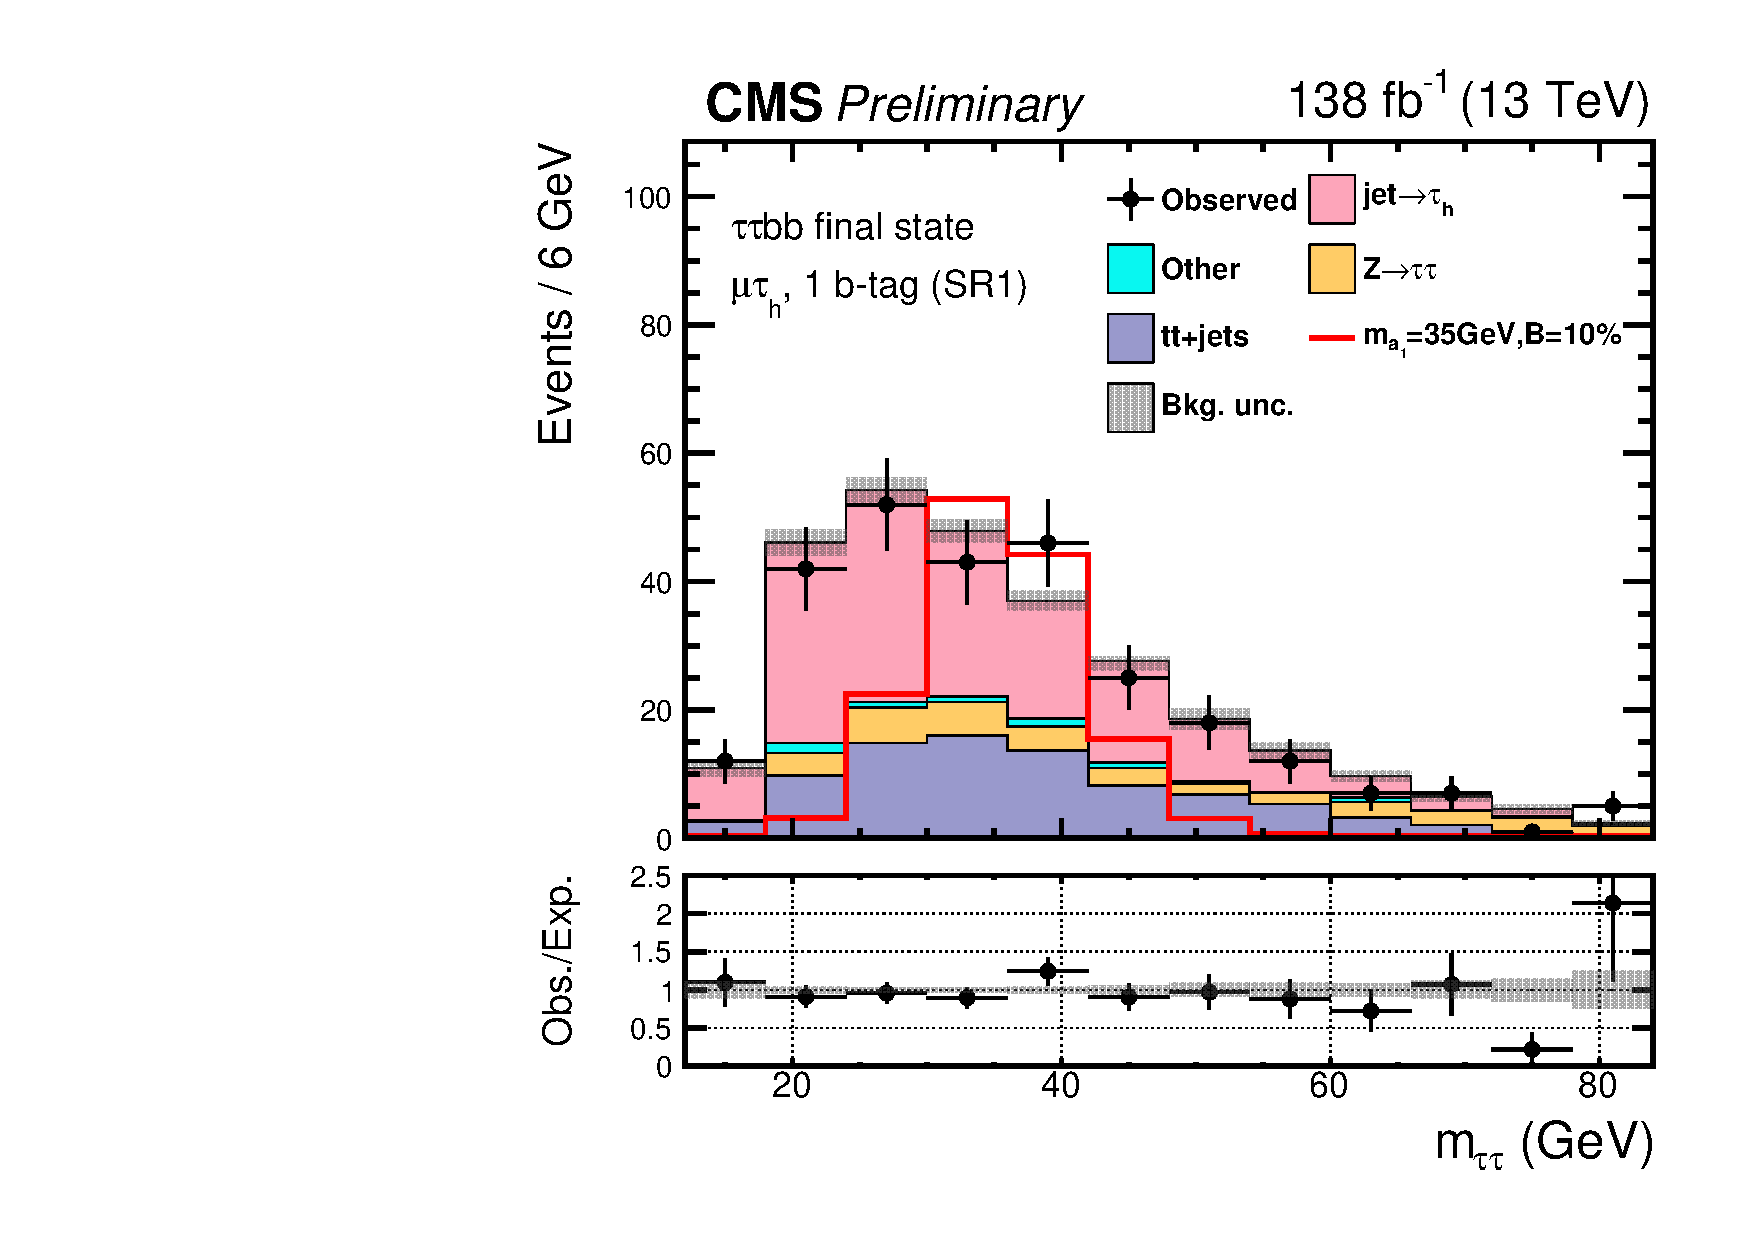
\includegraphics[width=0.32\textwidth]{figures/ch-14-results/mt_all_1_post_prelim-yes.pdf}
        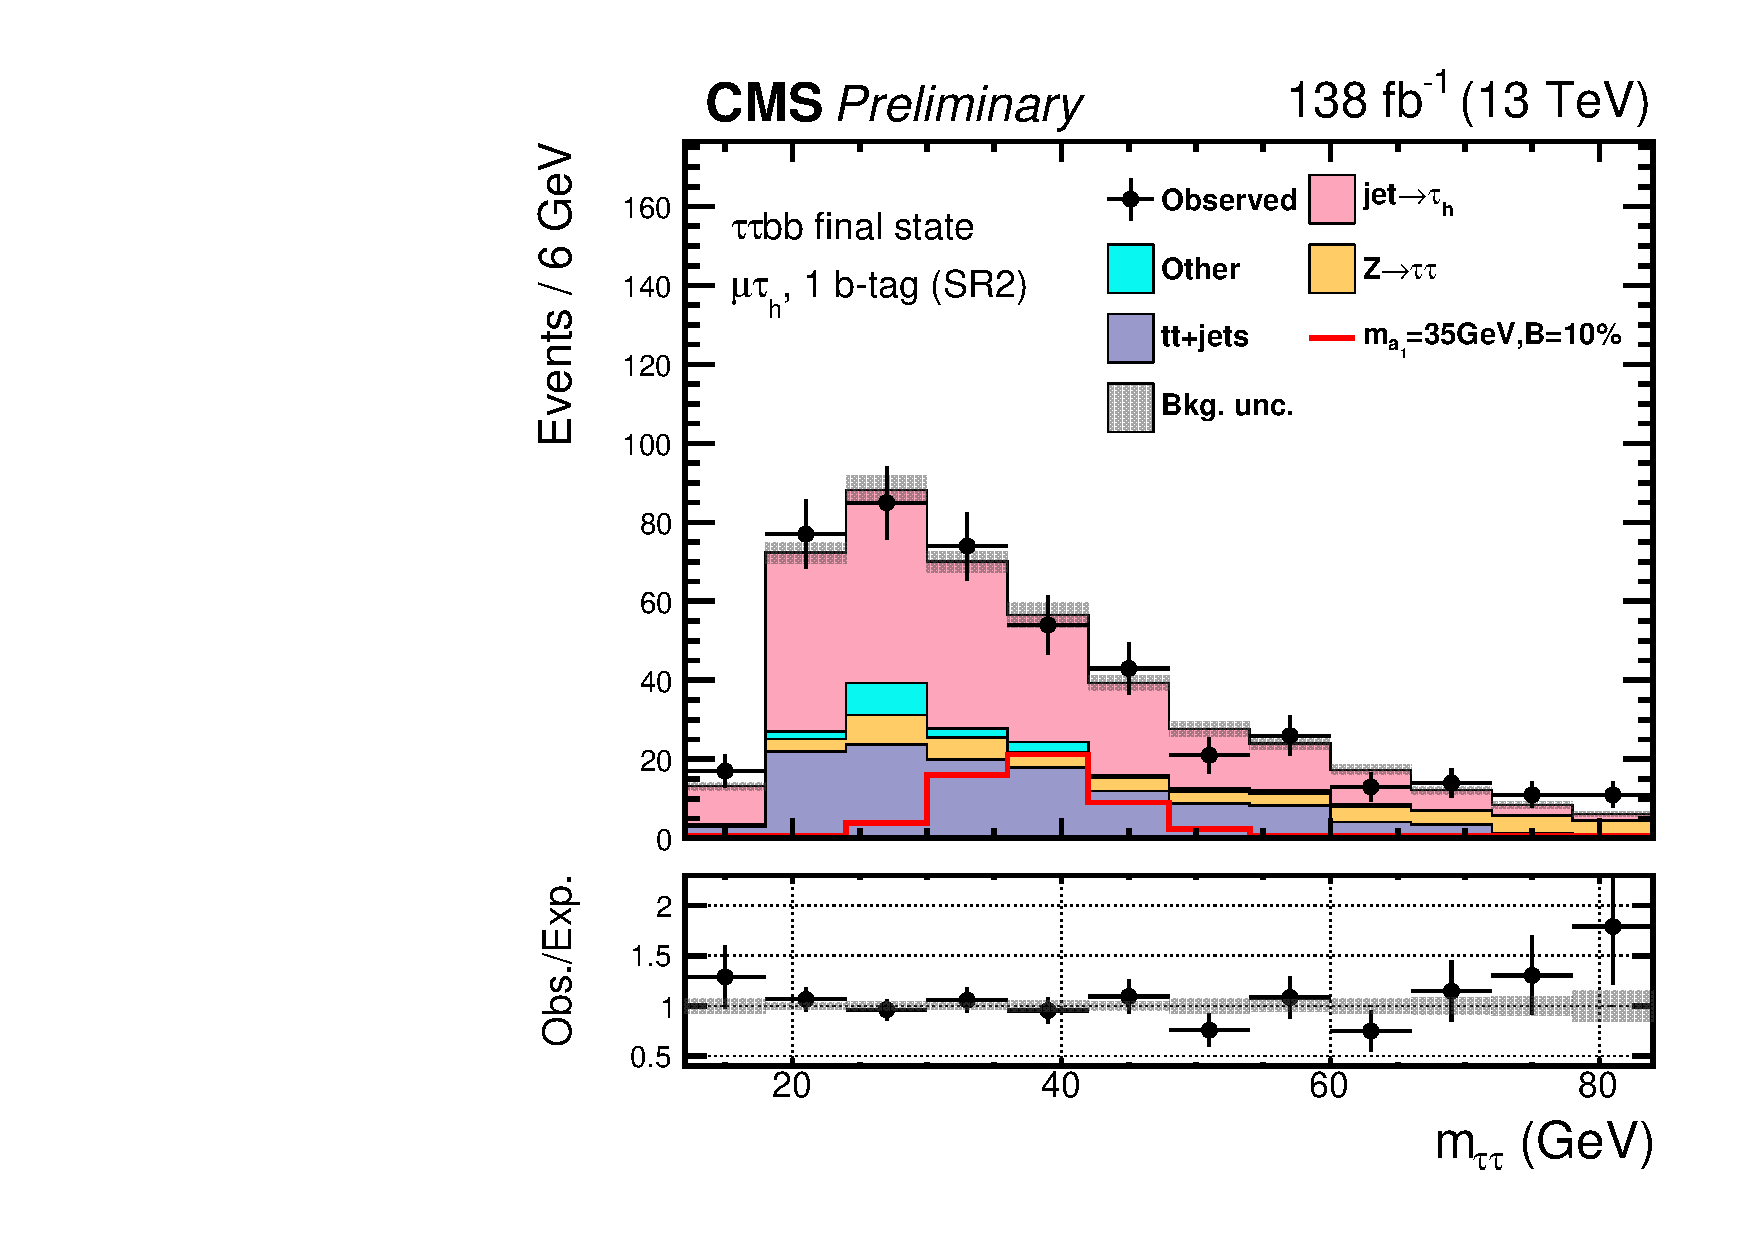
\includegraphics[width=0.32\textwidth]{figures/ch-14-results/mt_all_2_post_prelim-yes.pdf}
        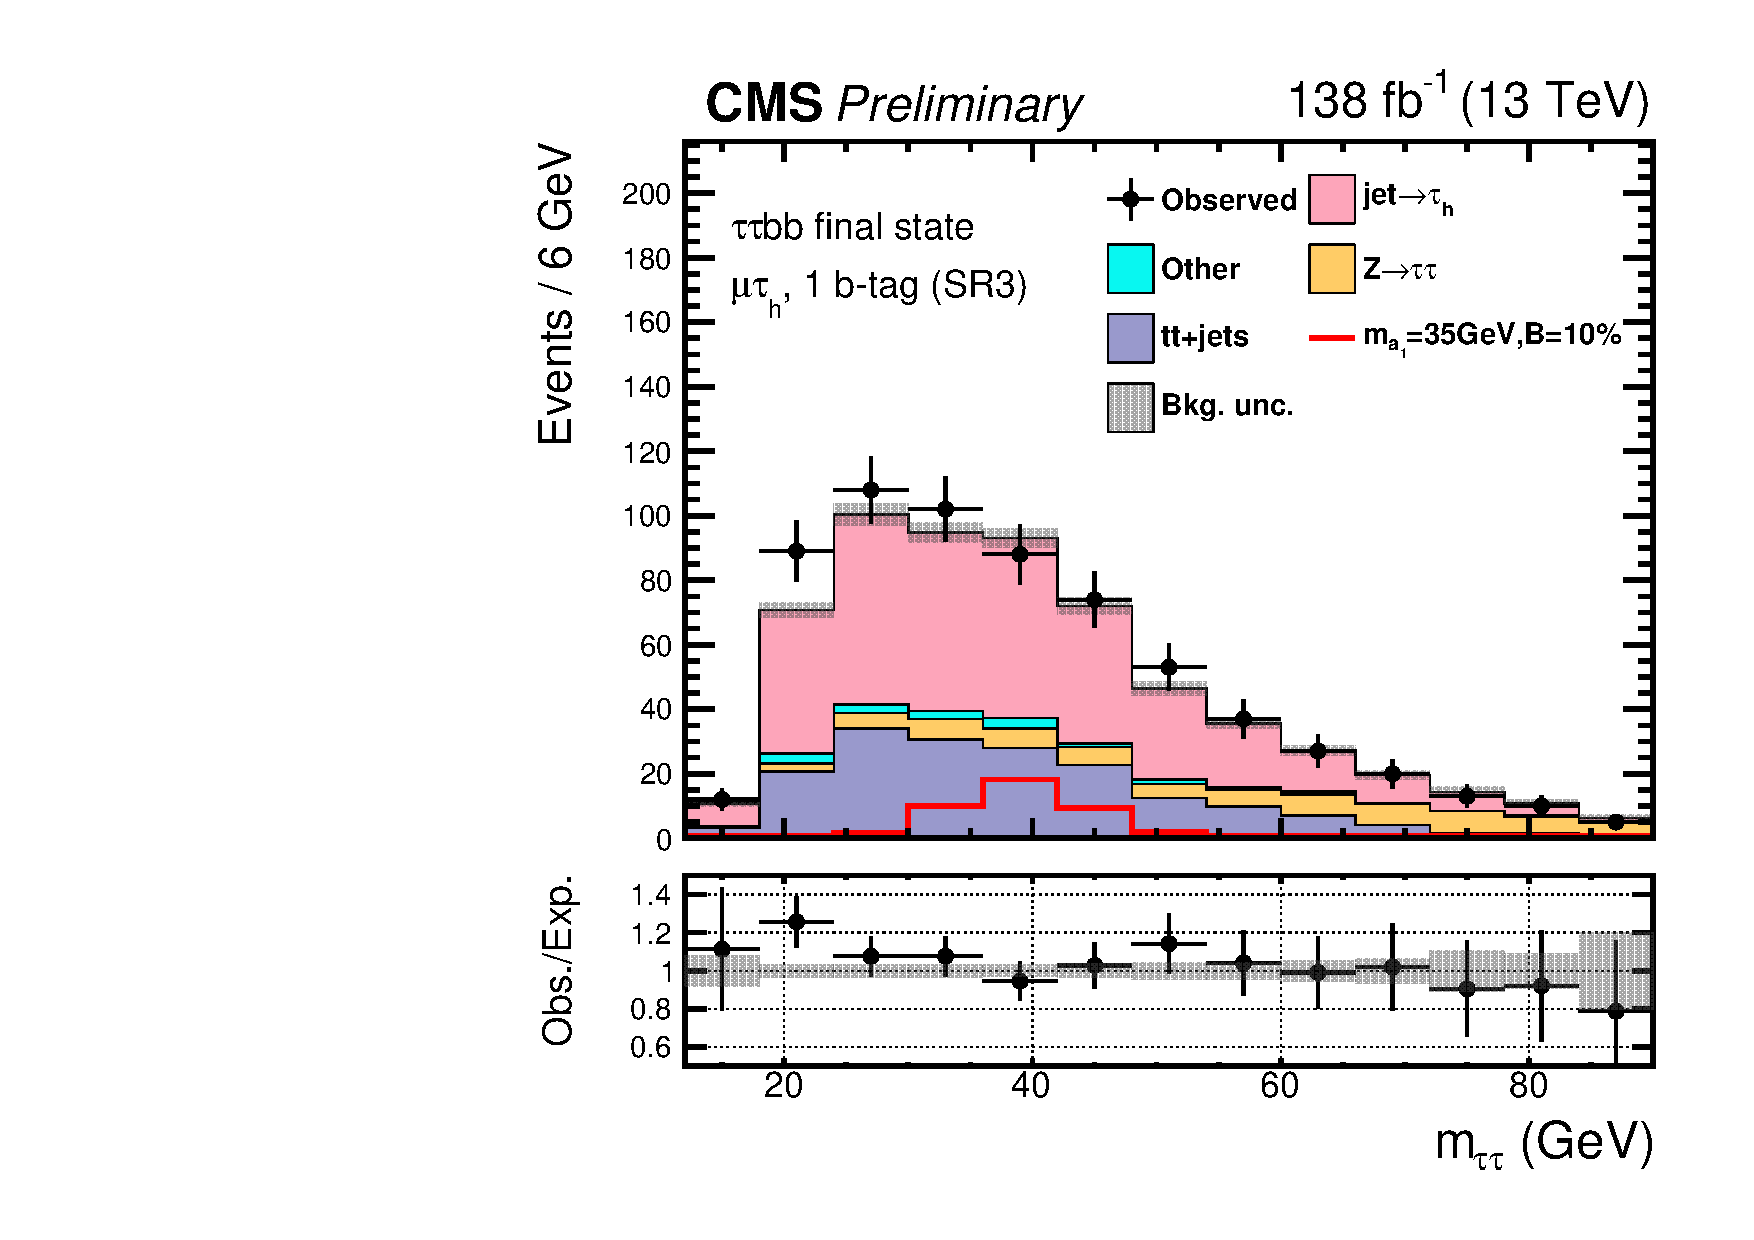
\includegraphics[width=0.32\textwidth]{figures/ch-14-results/mt_all_3_post_prelim-yes.pdf}\\
        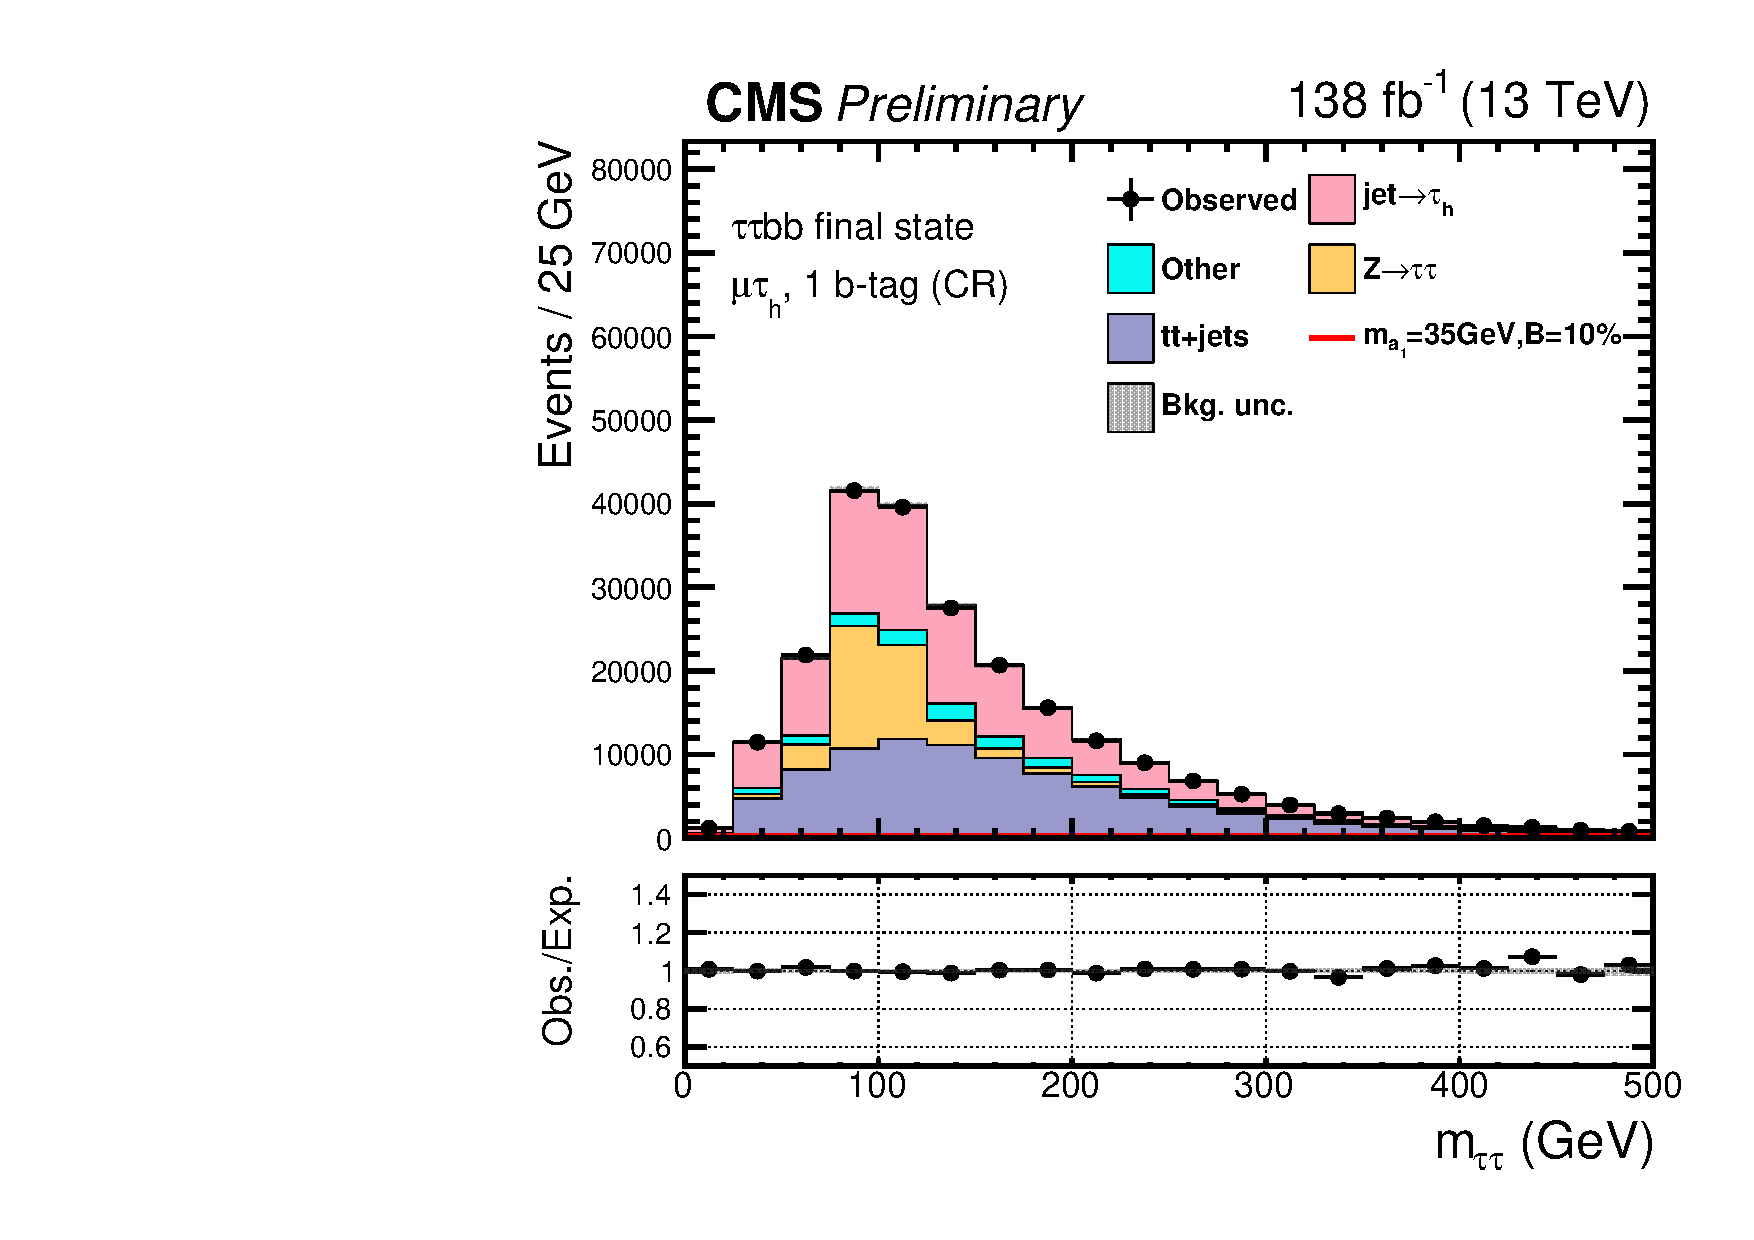
\includegraphics[width=0.32\textwidth]{figures/ch-14-results/mt_all_4_post_prelim-yes.pdf}
        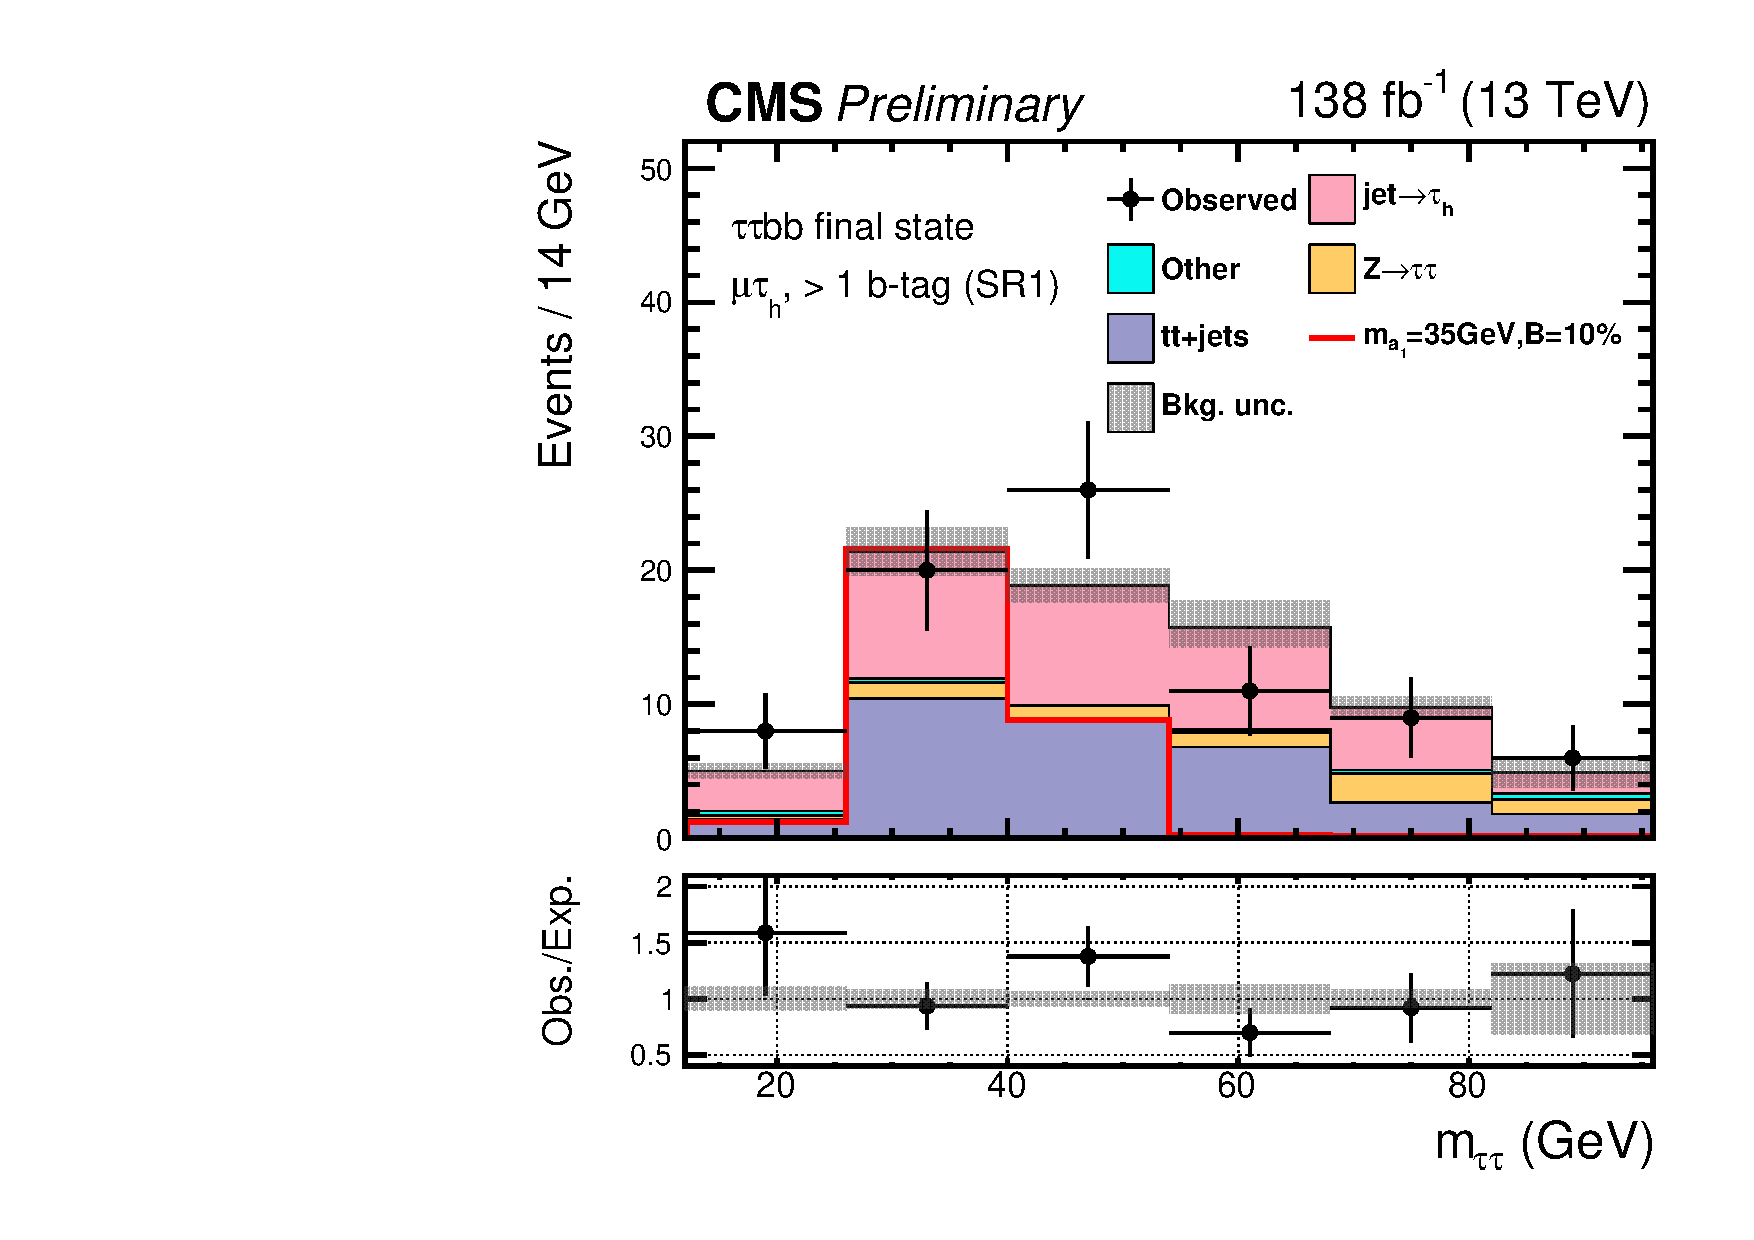
\includegraphics[width=0.32\textwidth]{figures/ch-14-results/mt_all_5_post_prelim-yes.pdf}
        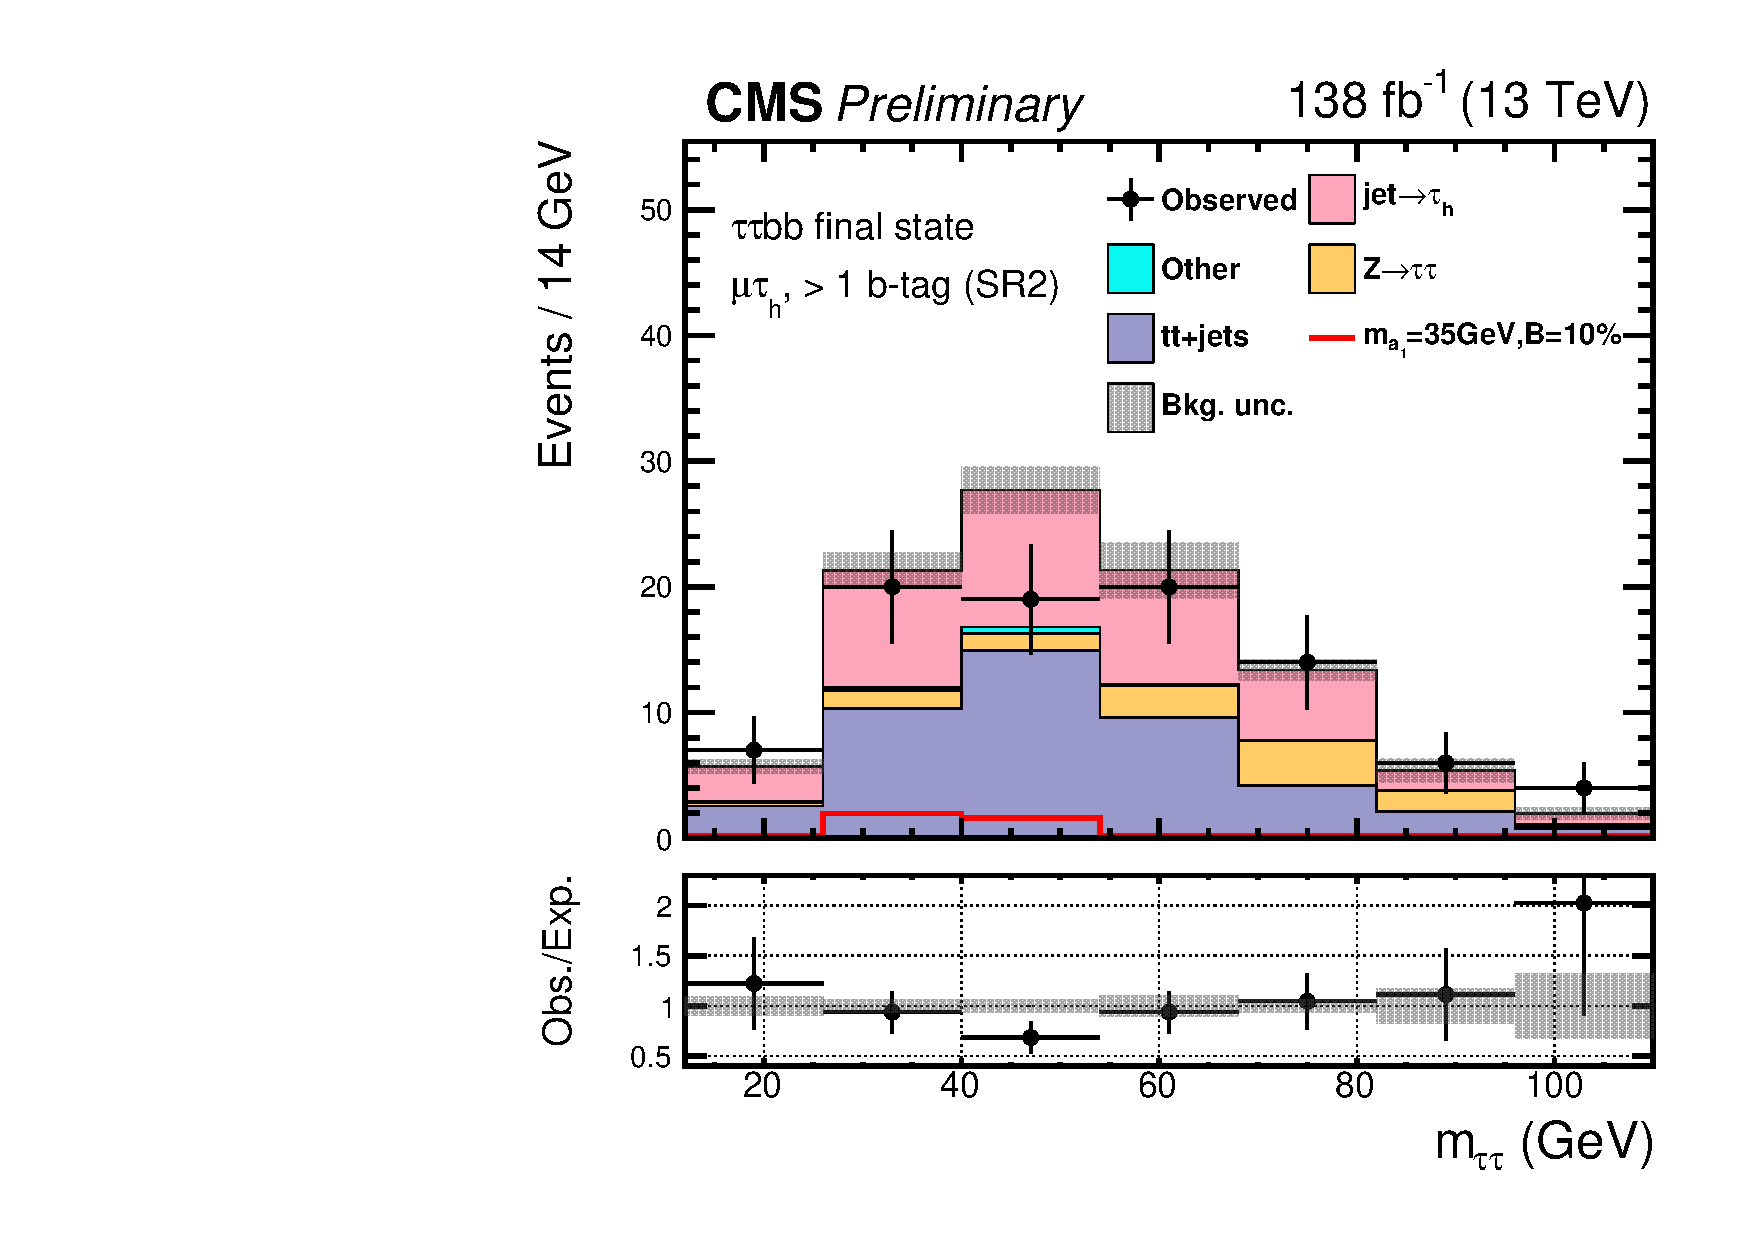
\includegraphics[width=0.32\textwidth]{figures/ch-14-results/mt_all_6_post_prelim-yes.pdf}\\
        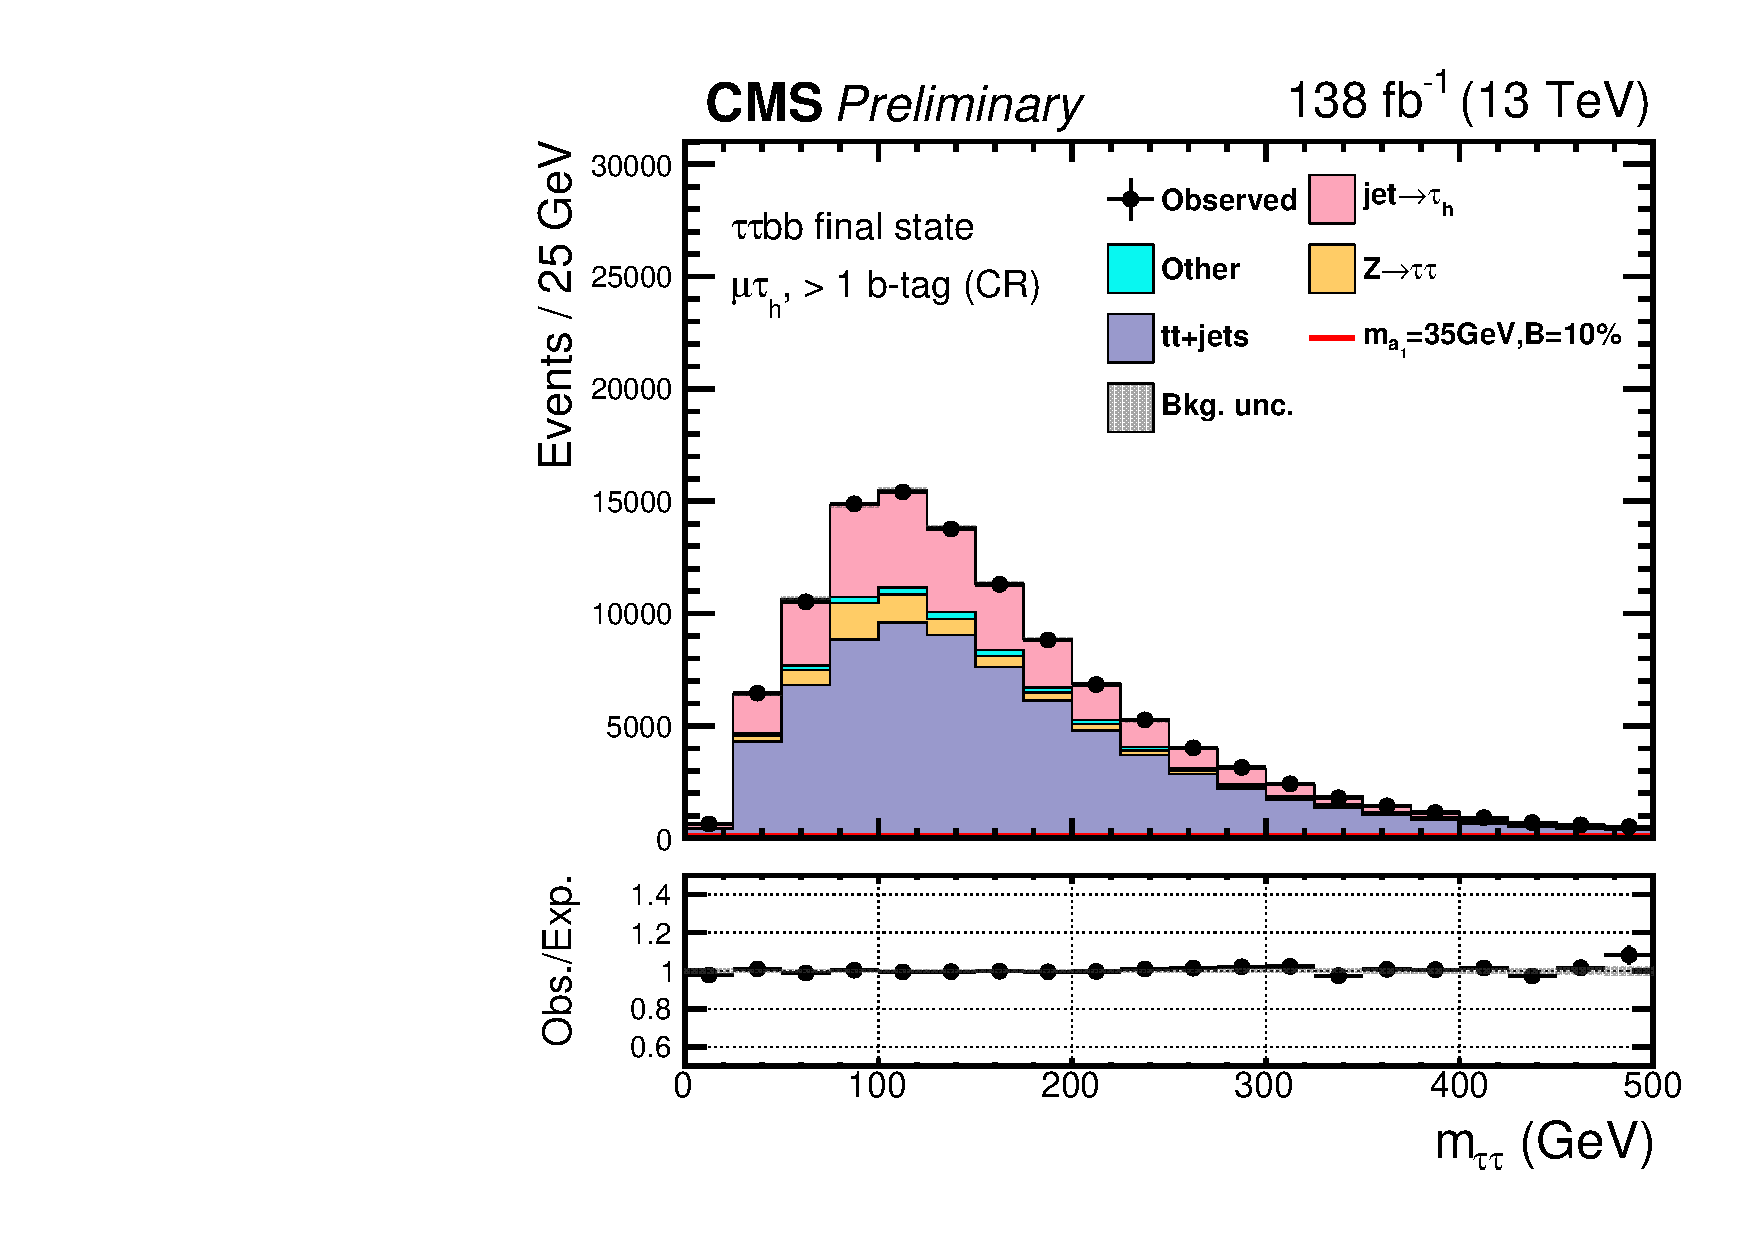
\includegraphics[width=0.32\textwidth]{figures/ch-14-results/mt_all_7_post_prelim-yes.pdf}
    \end{center}
    \caption[Postfit final $m_{\tau\tau}$ distributions in the $\mu\tau_{h}$ channel.]{Postfit final $m_{\tau\tau}$ distributions in the $\mu\tau_{h}$ channel \cite{CMS-AN-20-213}. Statistical and systematic uncertainties are included. \textit{Top row:} 1 b-tag jet categories: three signal regions (SR1, SR2, SR3). \textit{Middle row, left to right:} 1 b-tag jet categories: control region (CR), and 2 b-tag jet categories: two signal regions (SR1, SR2). \textit{Bottom:} 2 b-tag jet categories: control region (CR).}
    \label{fig:results_mtt_postfit_mtall}
\end{figure}

\begin{figure}[ht]
    \begin{center}
        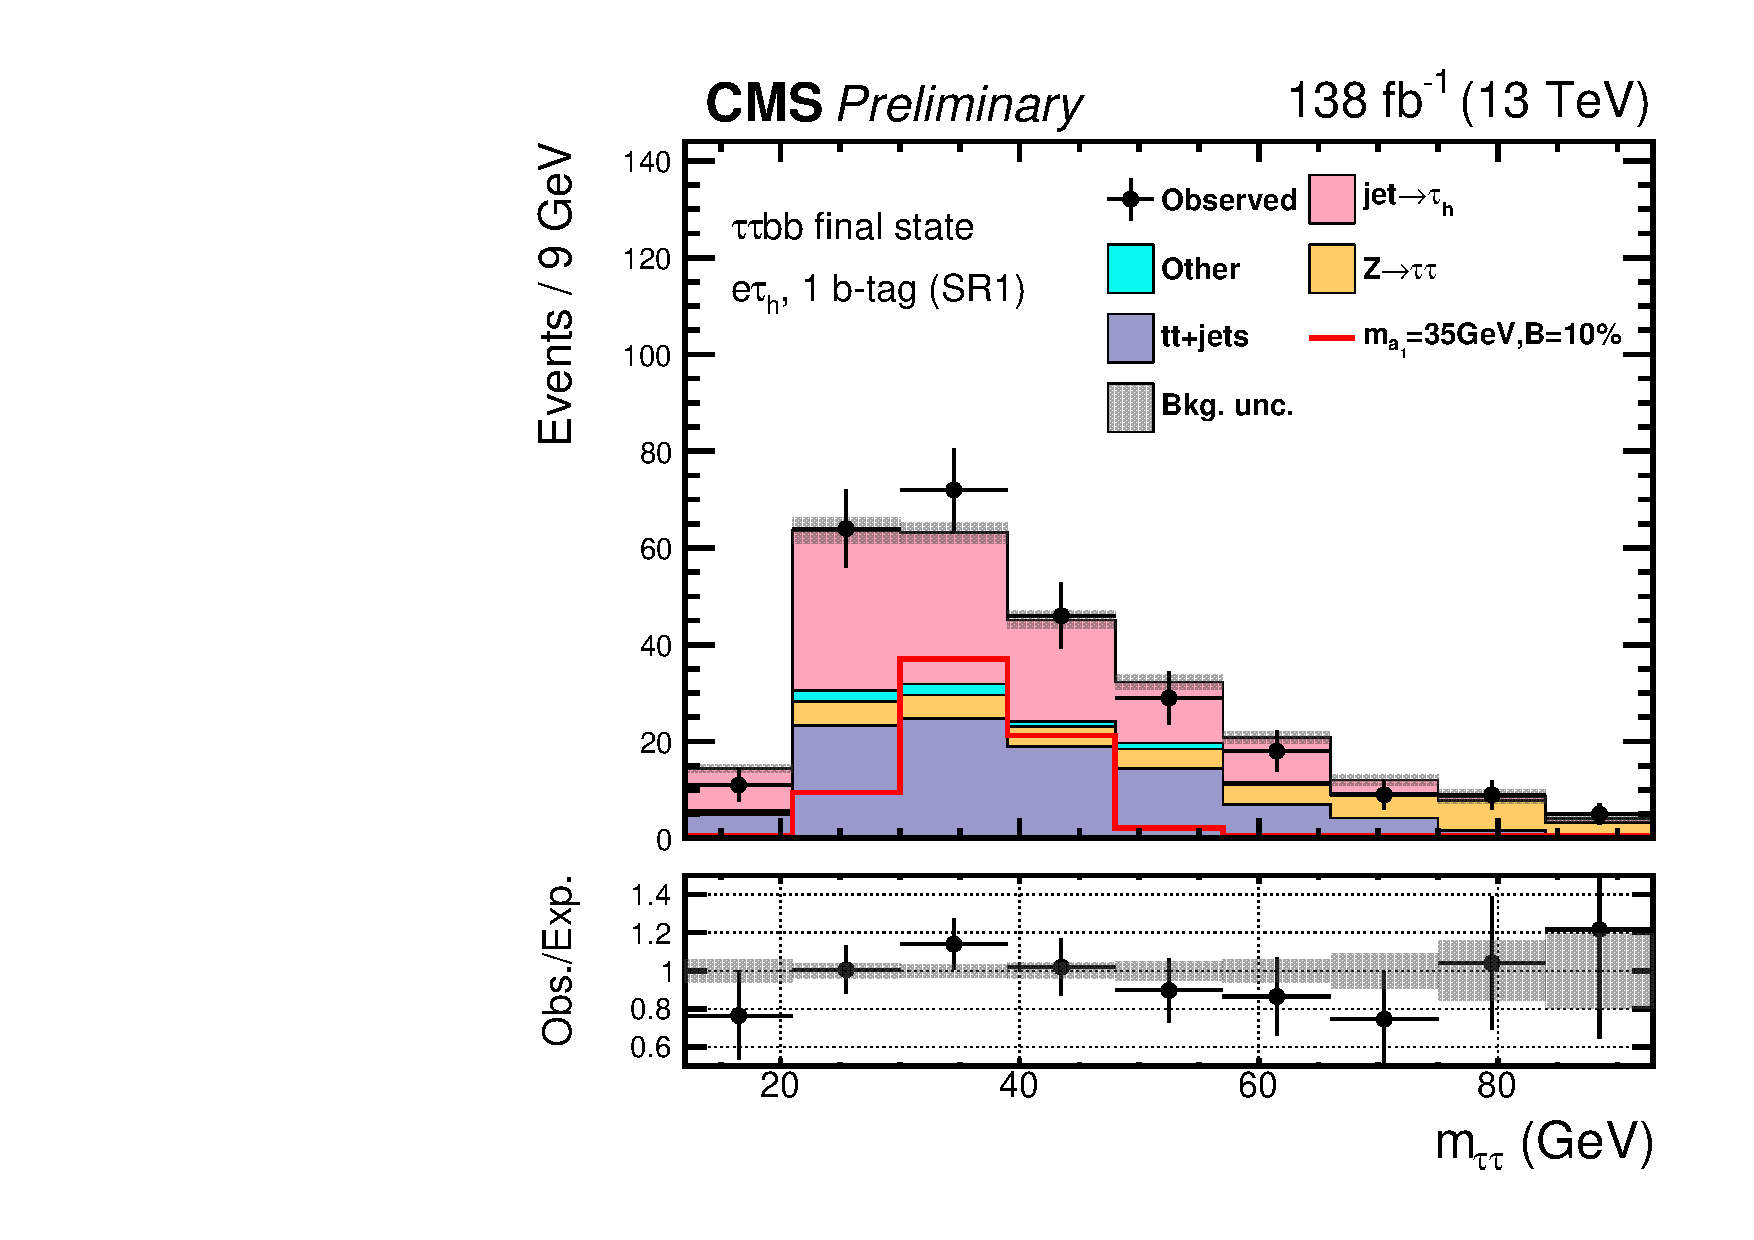
\includegraphics[width=0.32\textwidth]{figures/ch-14-results/et_all_1_post_prelim-yes.pdf}
        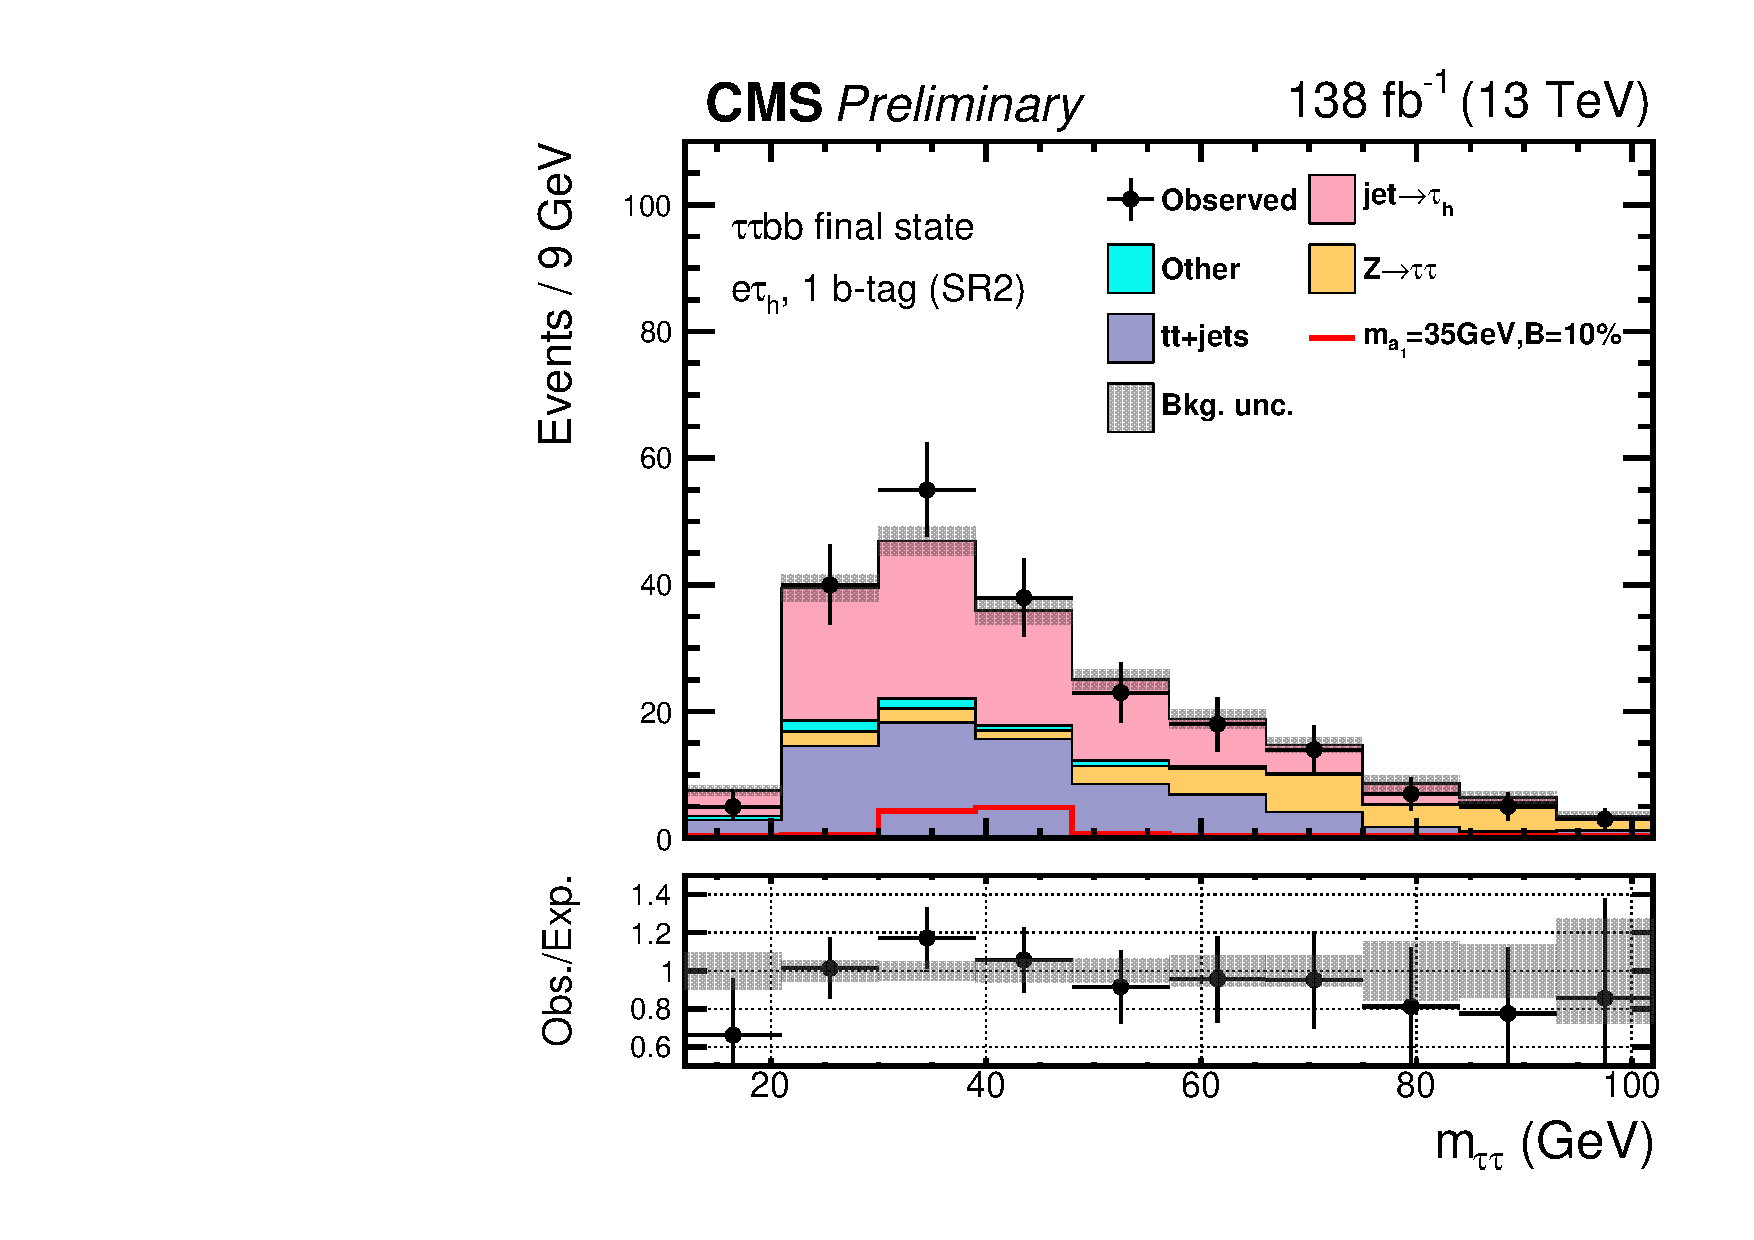
\includegraphics[width=0.32\textwidth]{figures/ch-14-results/et_all_2_post_prelim-yes.pdf}
        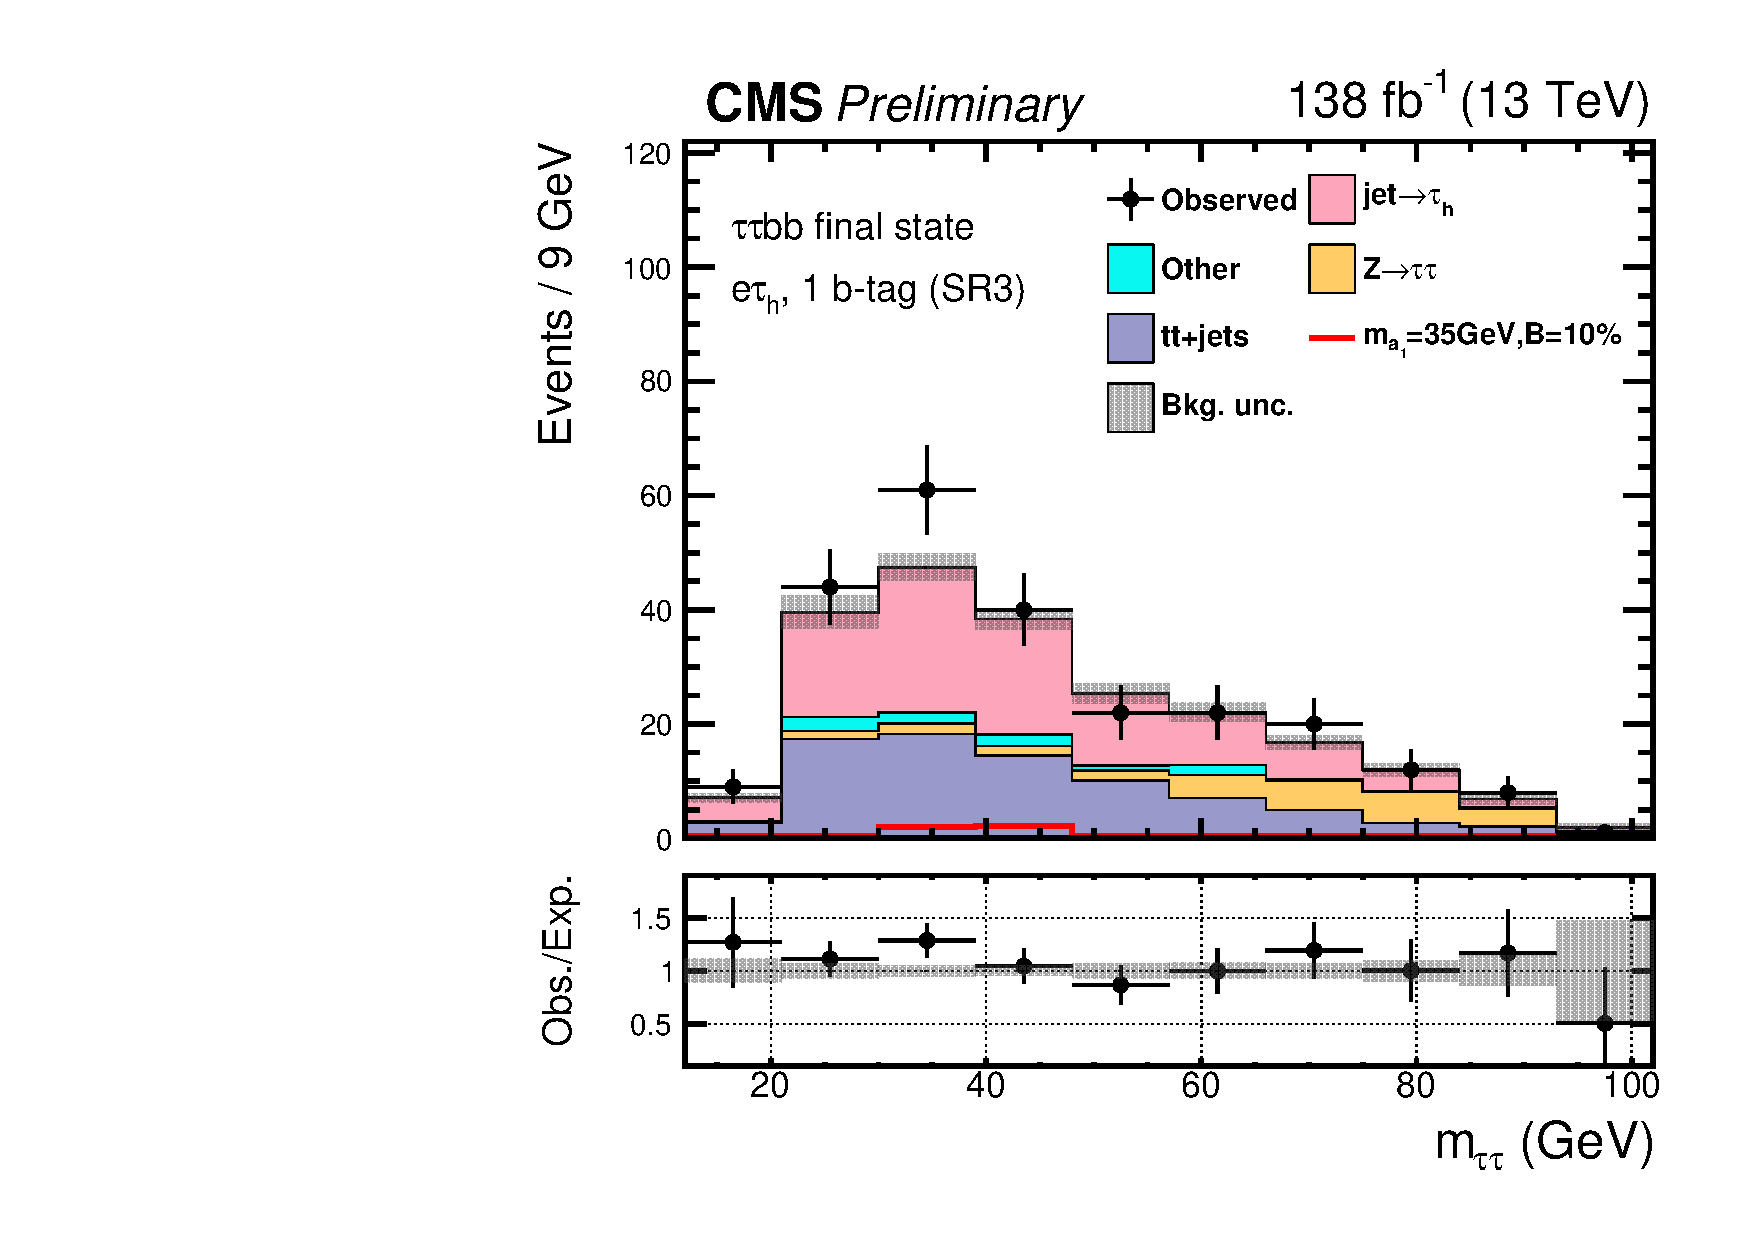
\includegraphics[width=0.32\textwidth]{figures/ch-14-results/et_all_3_post_prelim-yes.pdf}\\
        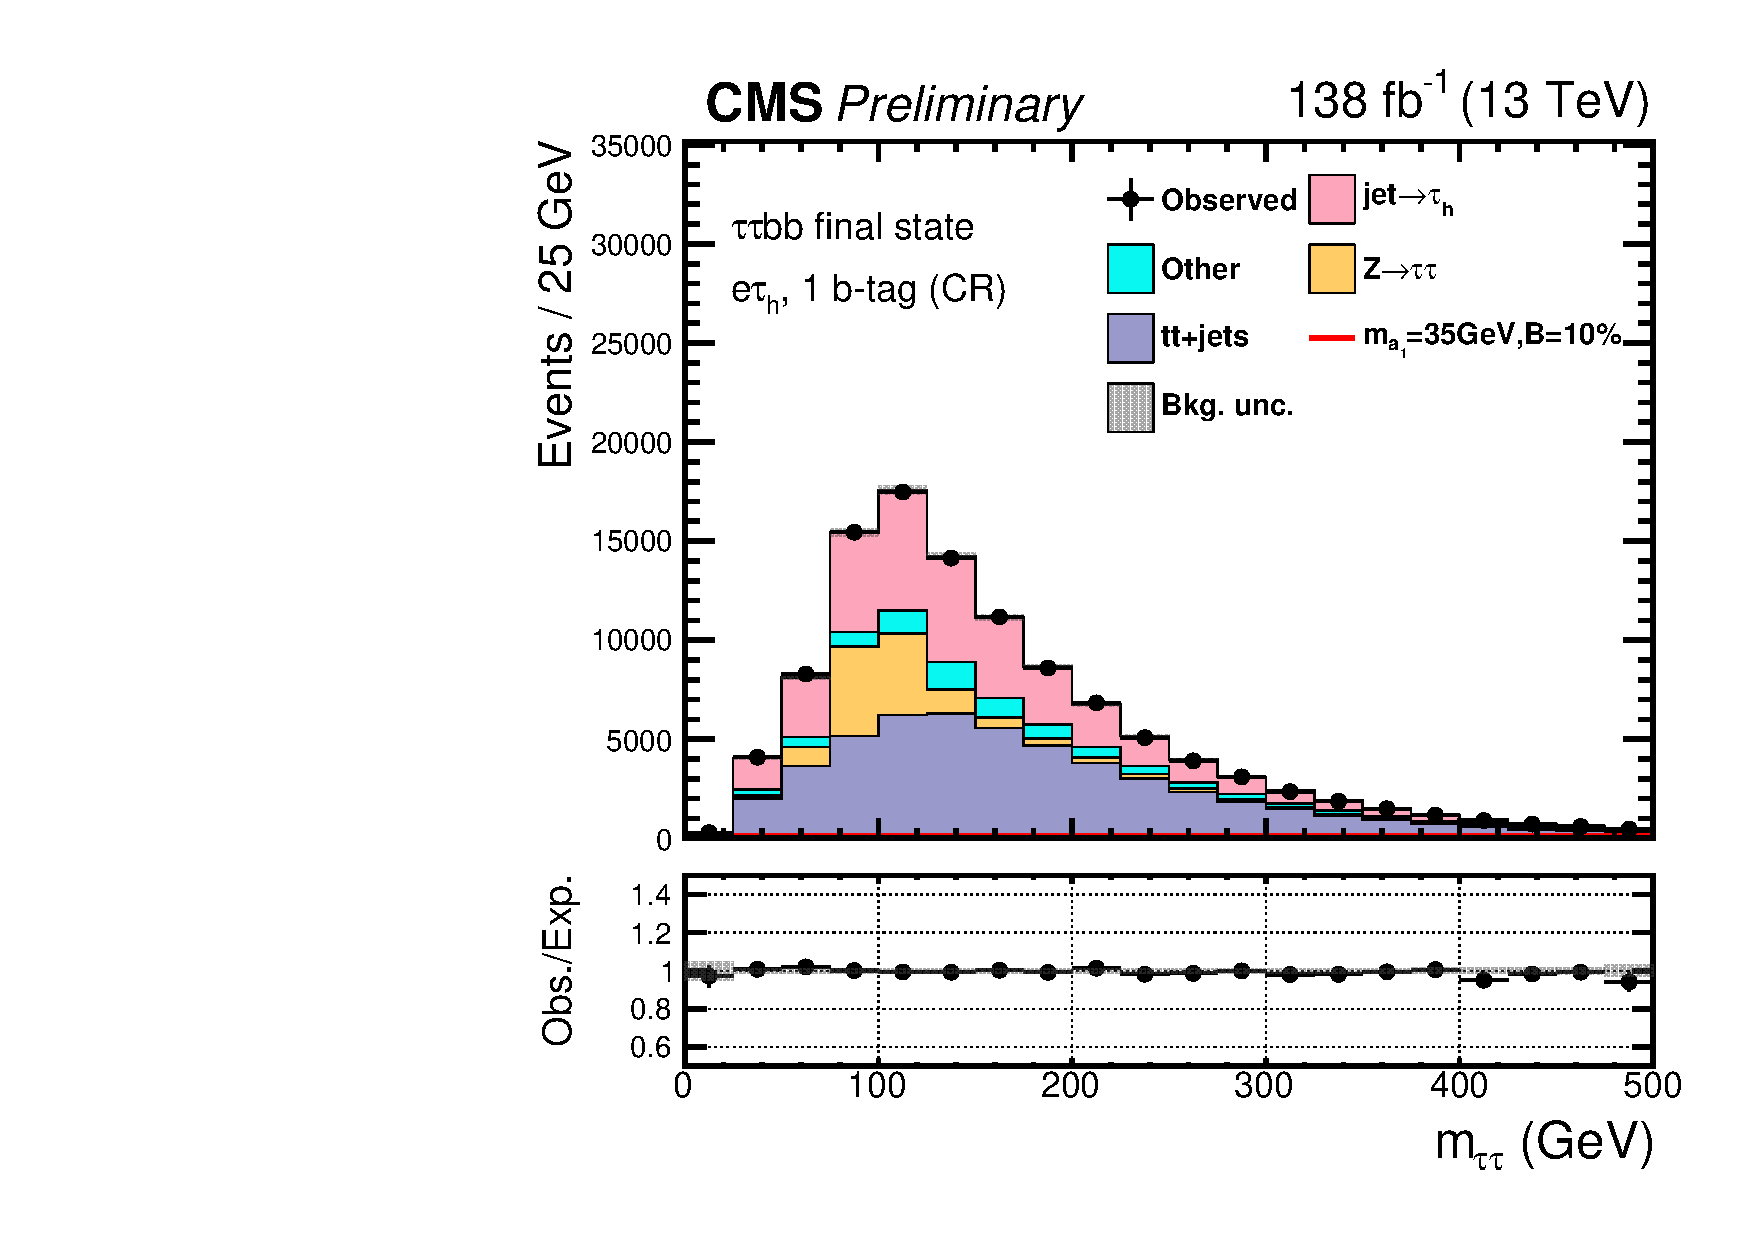
\includegraphics[width=0.32\textwidth]{figures/ch-14-results/et_all_4_post_prelim-yes.pdf}
        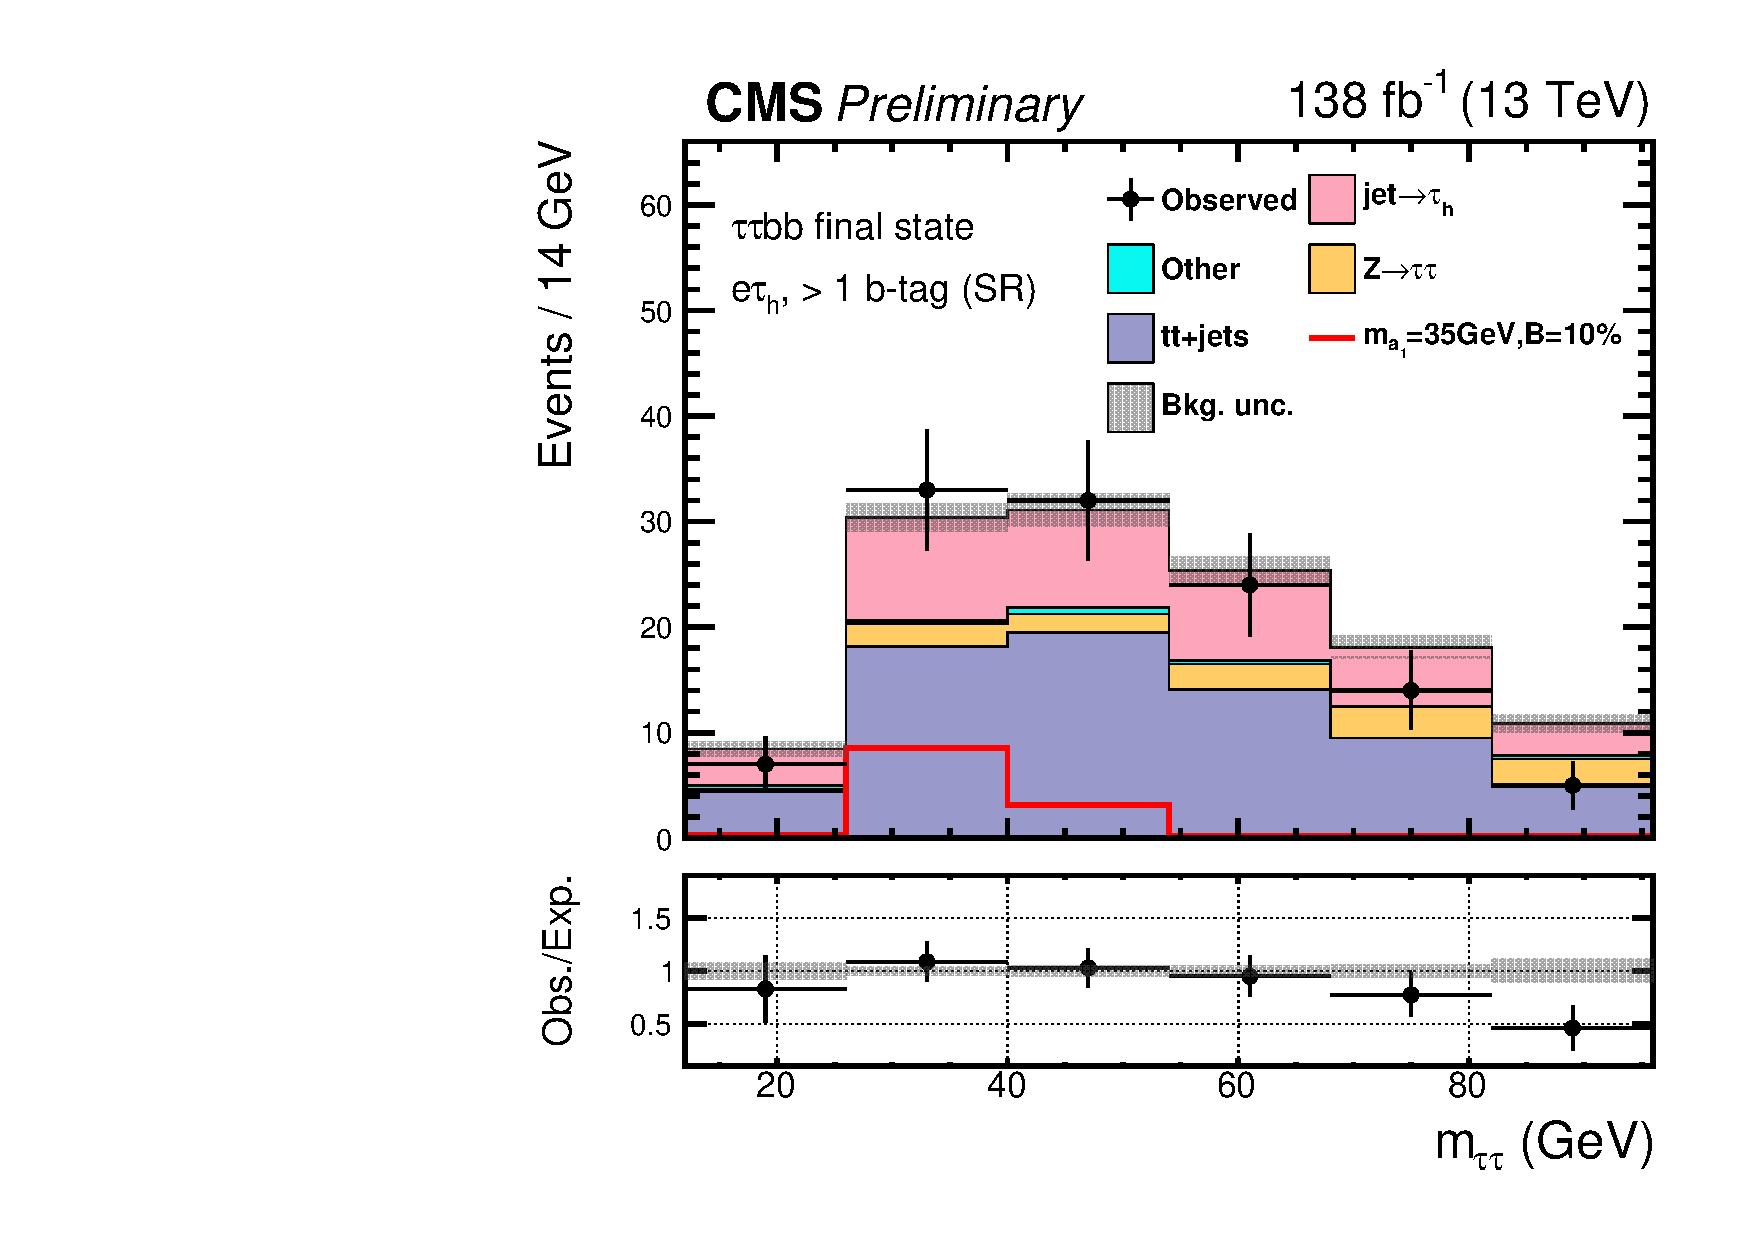
\includegraphics[width=0.32\textwidth]{figures/ch-14-results/et_all_5_post_prelim-yes.pdf}
        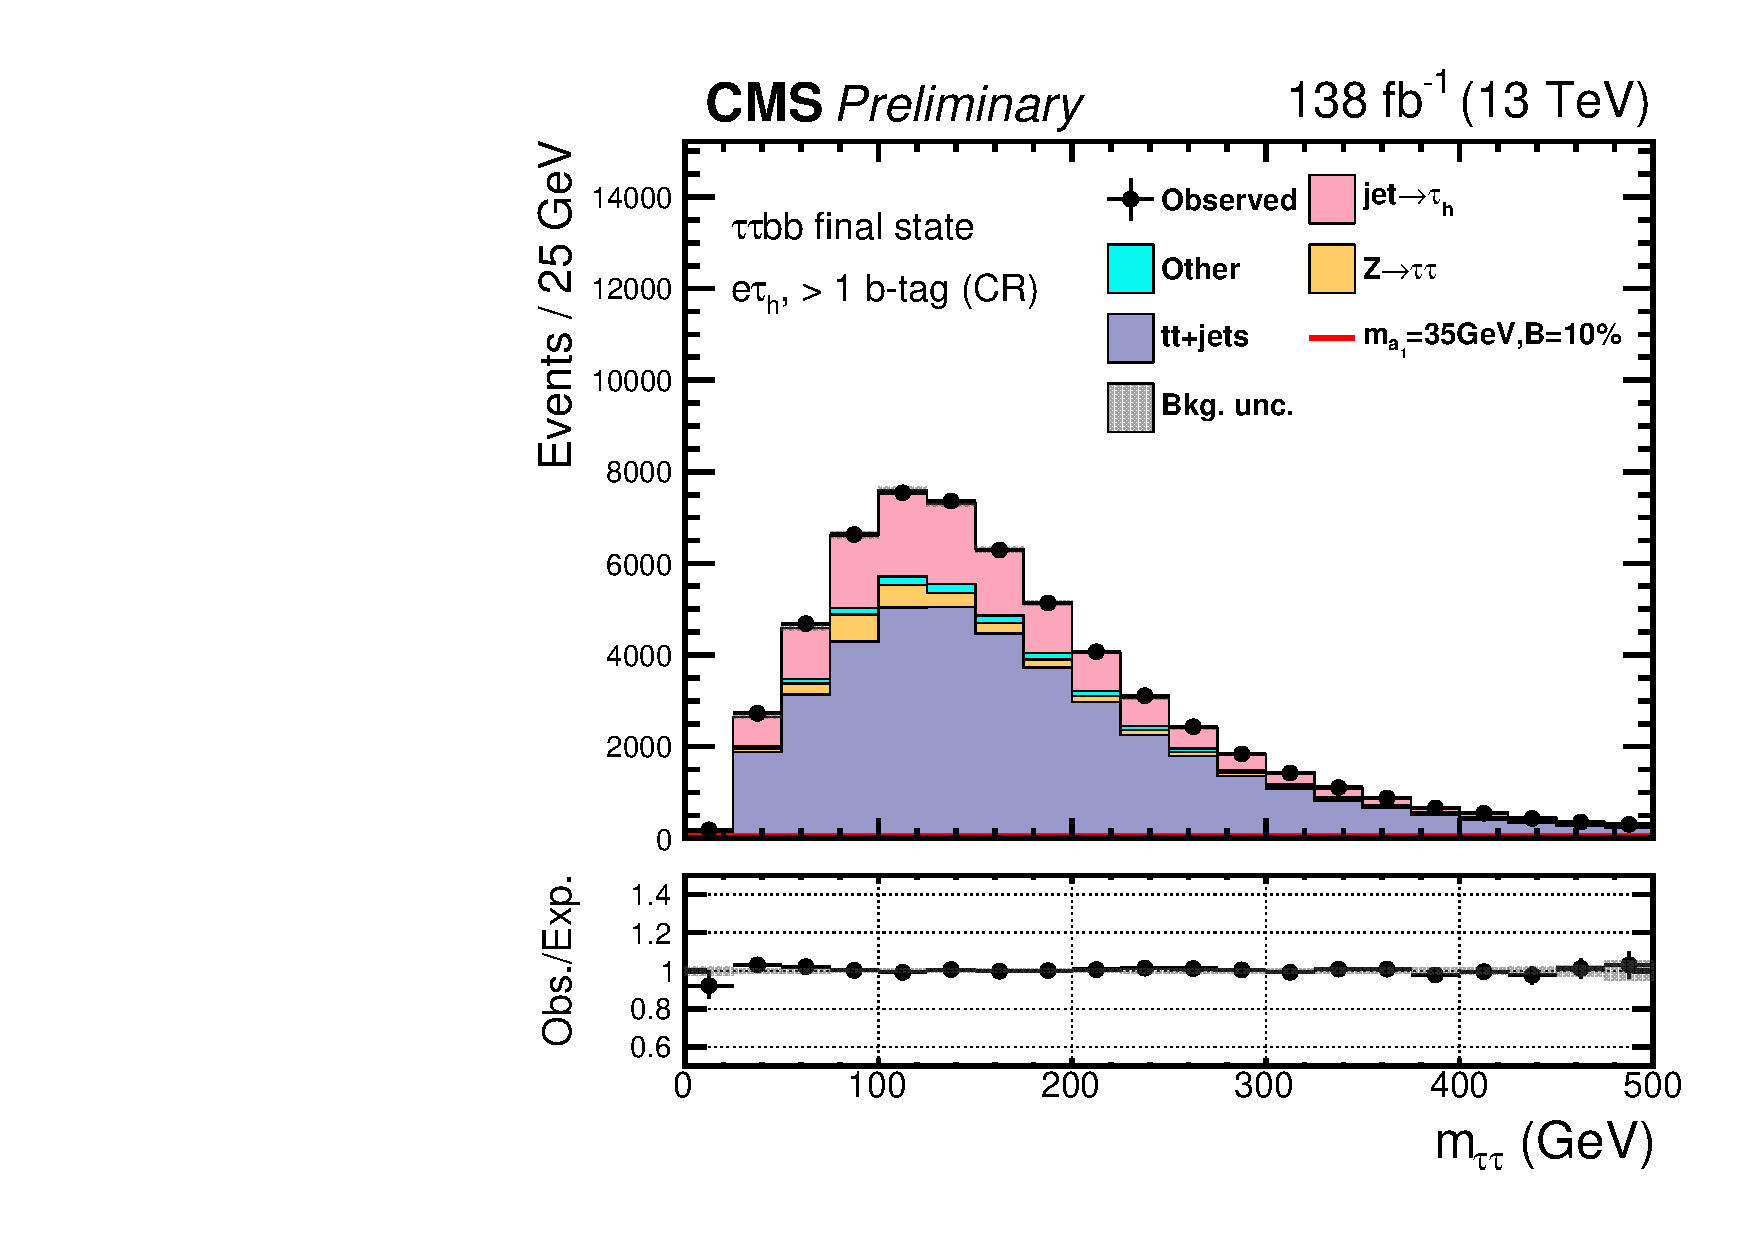
\includegraphics[width=0.32\textwidth]{figures/ch-14-results/et_all_6_post_prelim-yes.pdf}
    \end{center}
    \caption[Postfit final $m_{\tau\tau}$ distributions in the $e\tau_{h}$ channel]{Postfit final $m_{\tau\tau}$ distributions in the $e\tau_{h}$ channel \cite{CMS-AN-20-213}. Statistical and systematic uncertainties are included. \textit{Top row:} 1 b-tag jet categories: three signal regions (SR1, SR2, SR3). \textit{Bottom row, left to right:} 1 b-tag jet categories: control region (CR), and 2 b-tag jet categories: signal region (SR) and control region (CR).}
    \label{fig:results_mtt_postfit_etall}
\end{figure}

\begin{figure}[ht]
    \begin{center}
        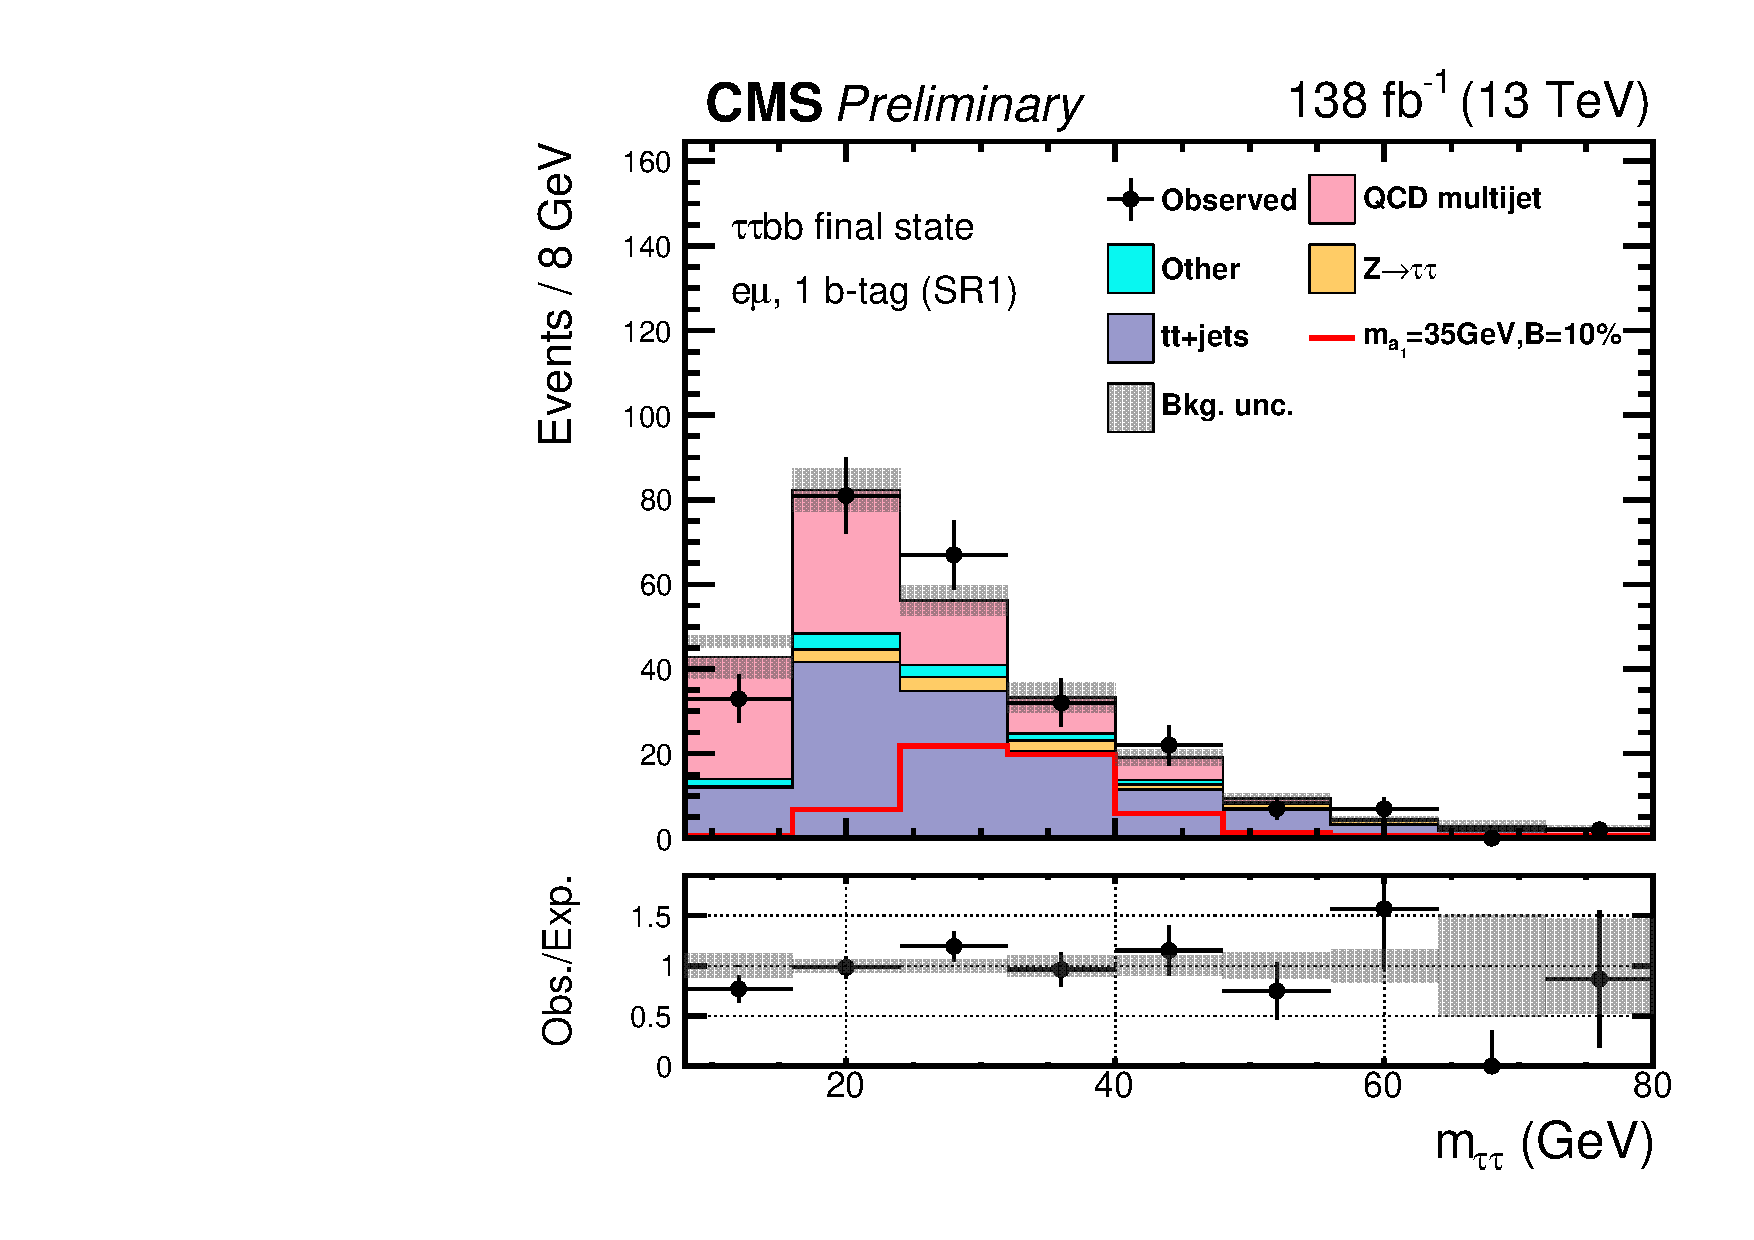
\includegraphics[width=0.32\textwidth]{figures/ch-14-results/em_all_1_post_prelim-yes.pdf}
        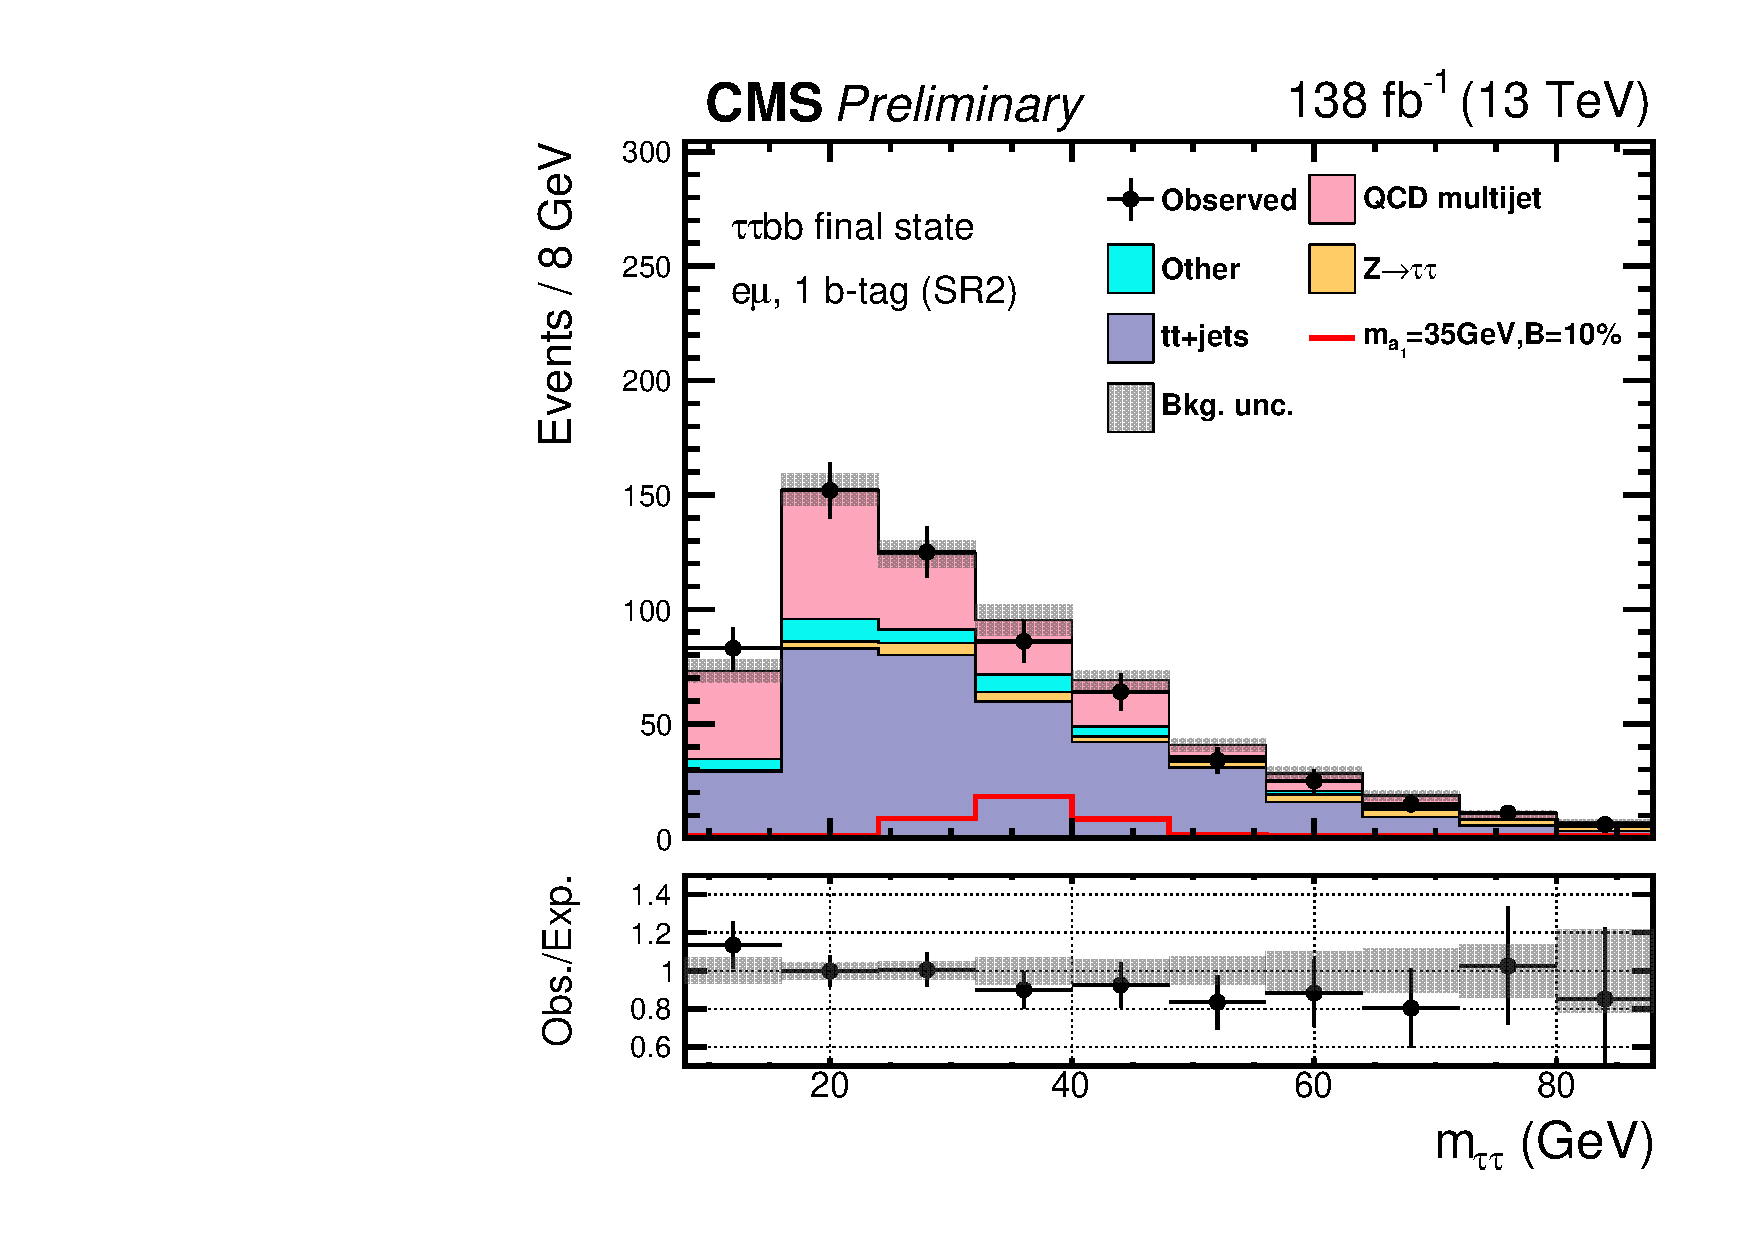
\includegraphics[width=0.32\textwidth]{figures/ch-14-results/em_all_2_post_prelim-yes.pdf}
        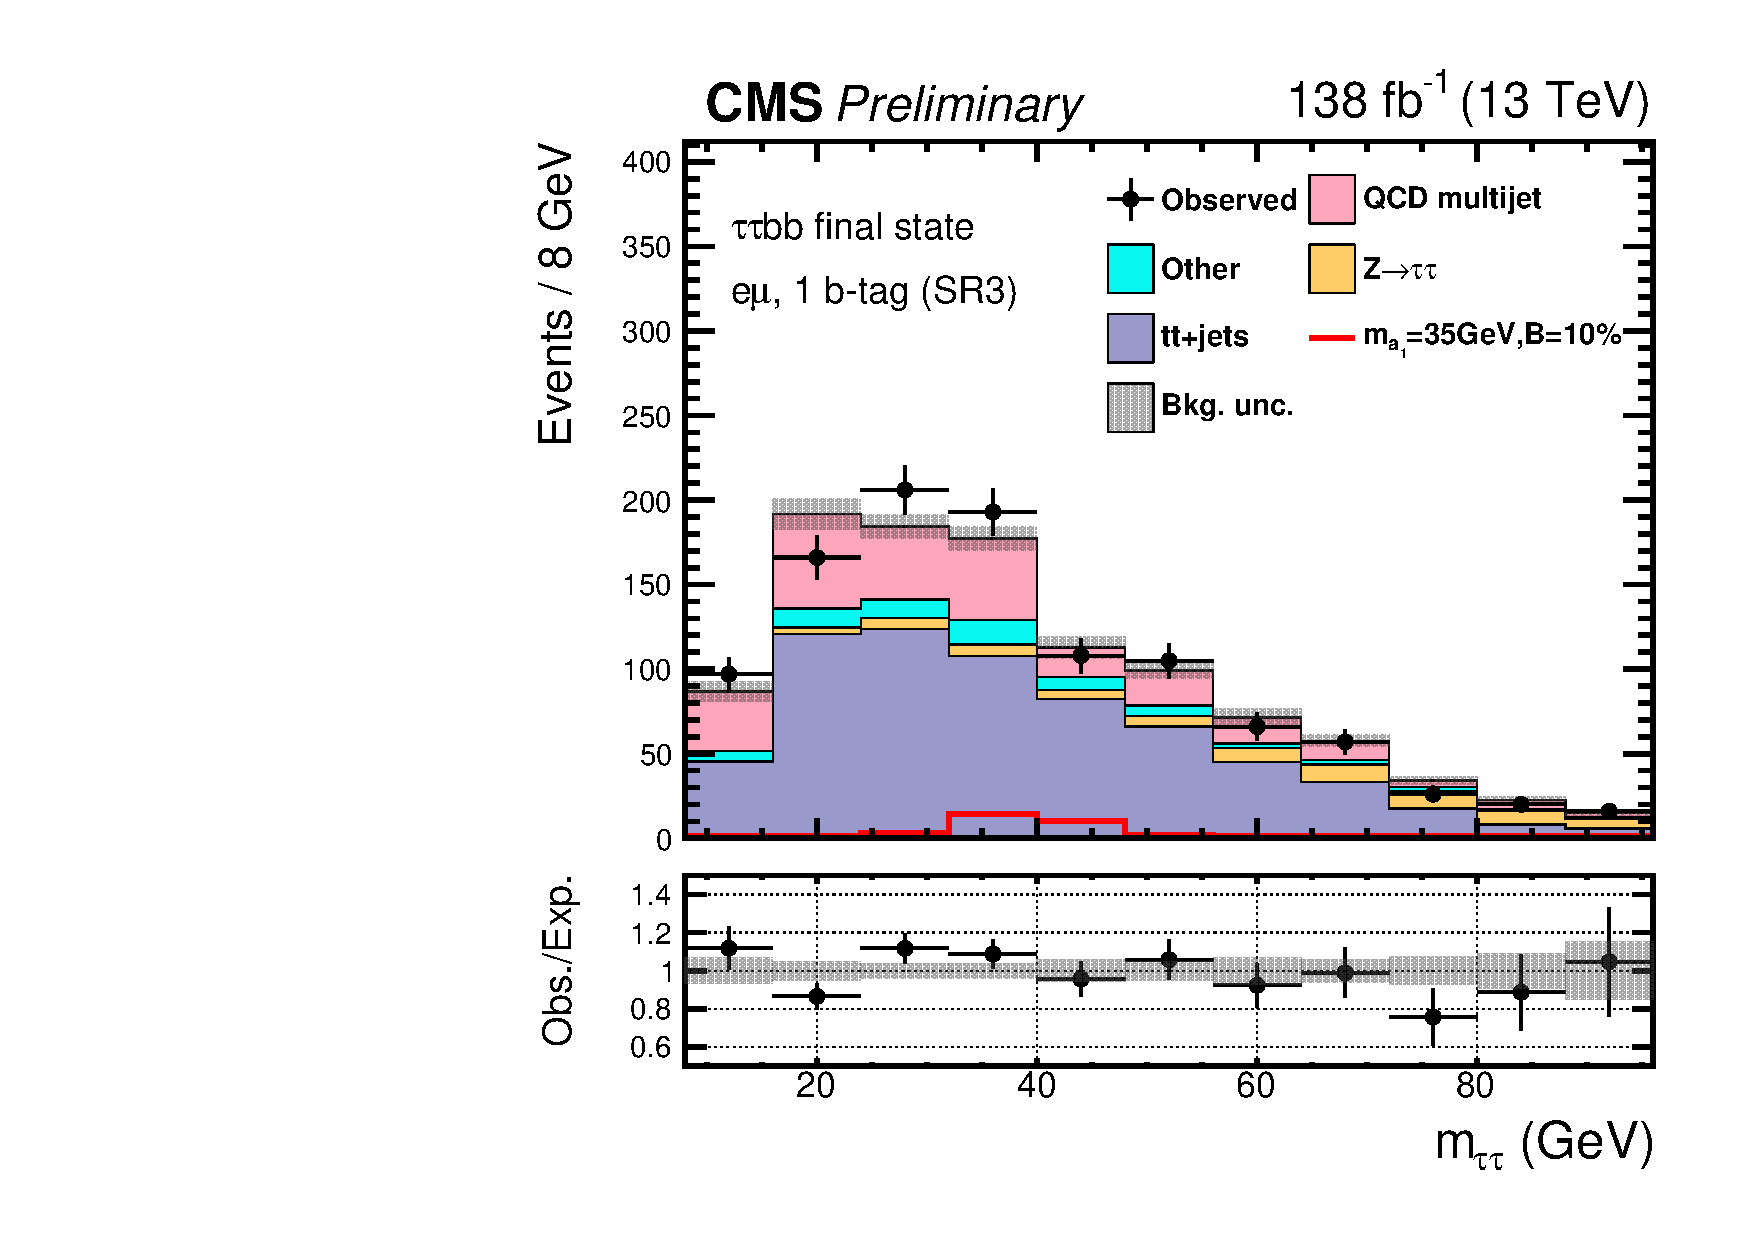
\includegraphics[width=0.32\textwidth]{figures/ch-14-results/em_all_3_post_prelim-yes.pdf}\\
        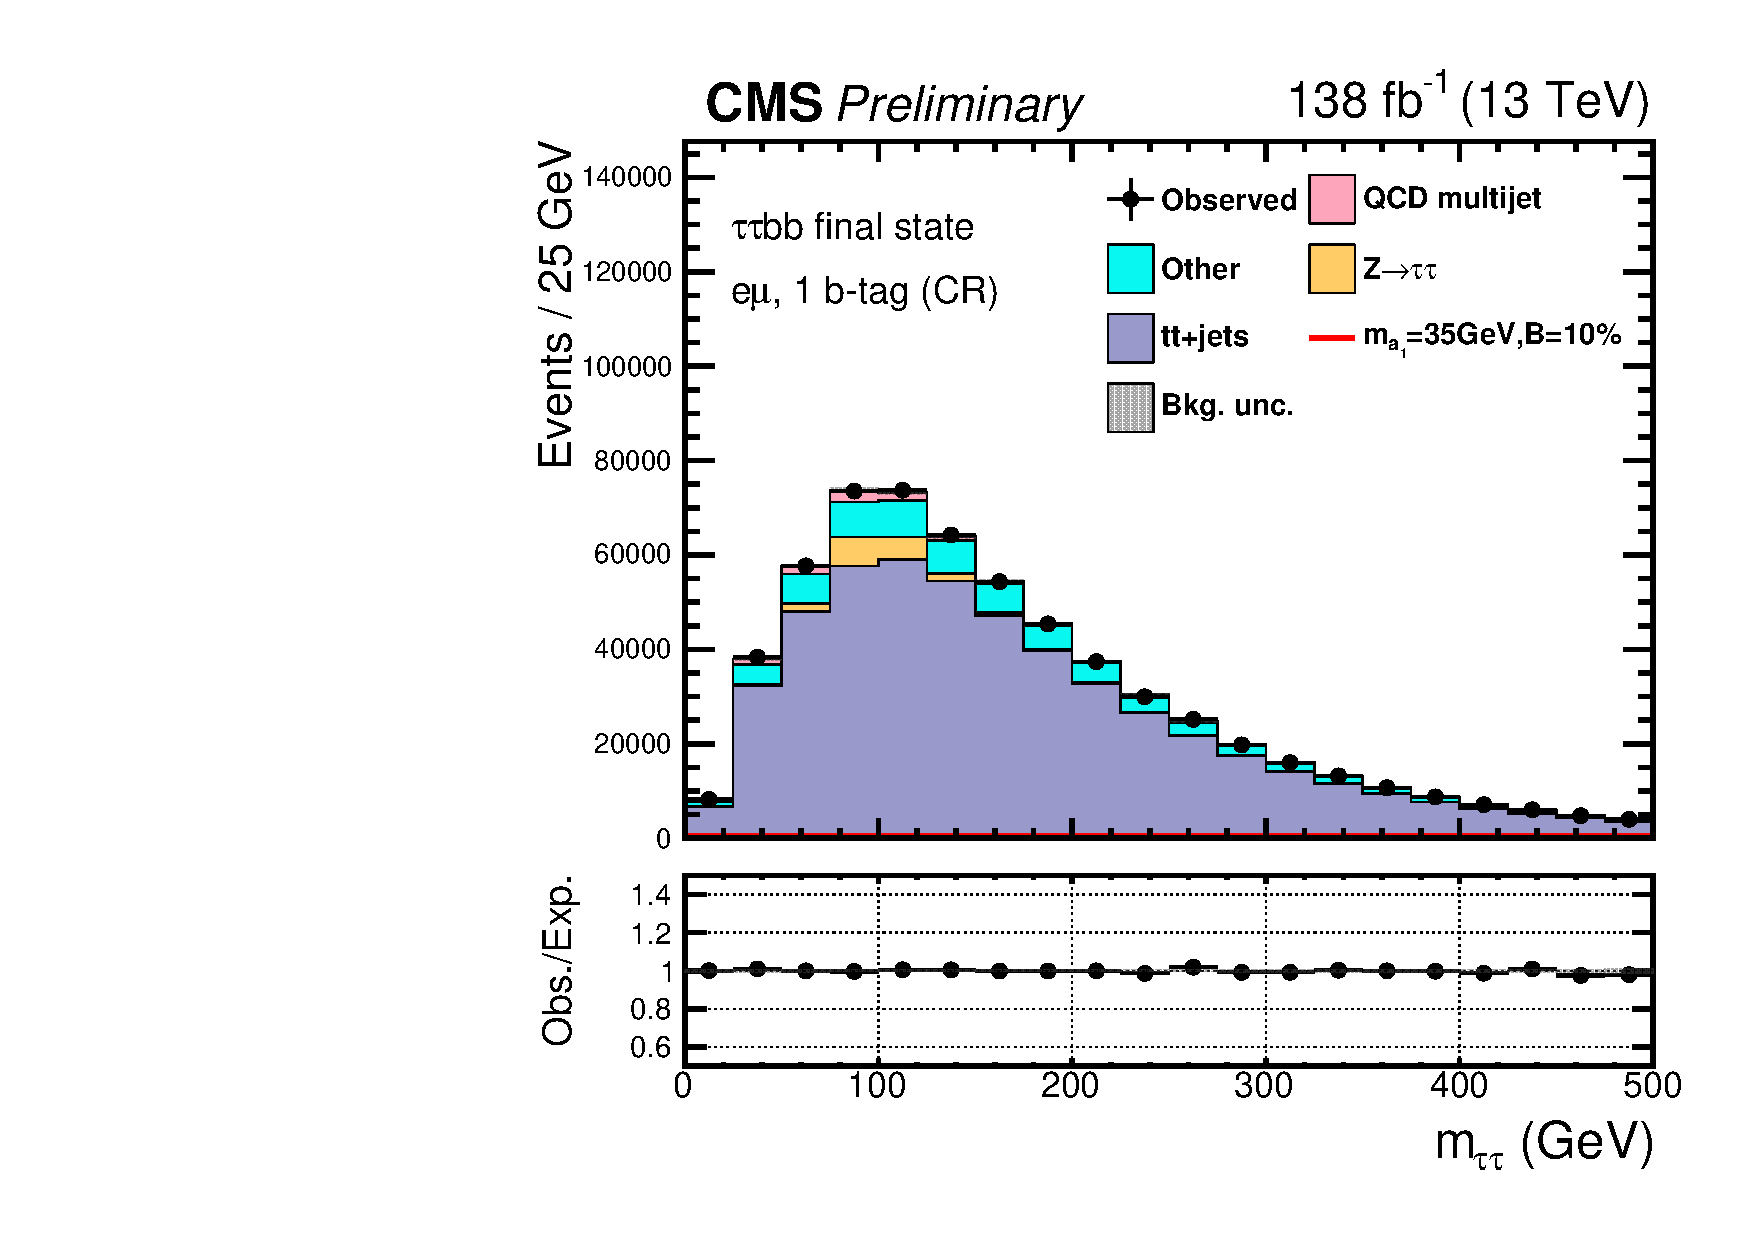
\includegraphics[width=0.32\textwidth]{figures/ch-14-results/em_all_4_post_prelim-yes.pdf}
        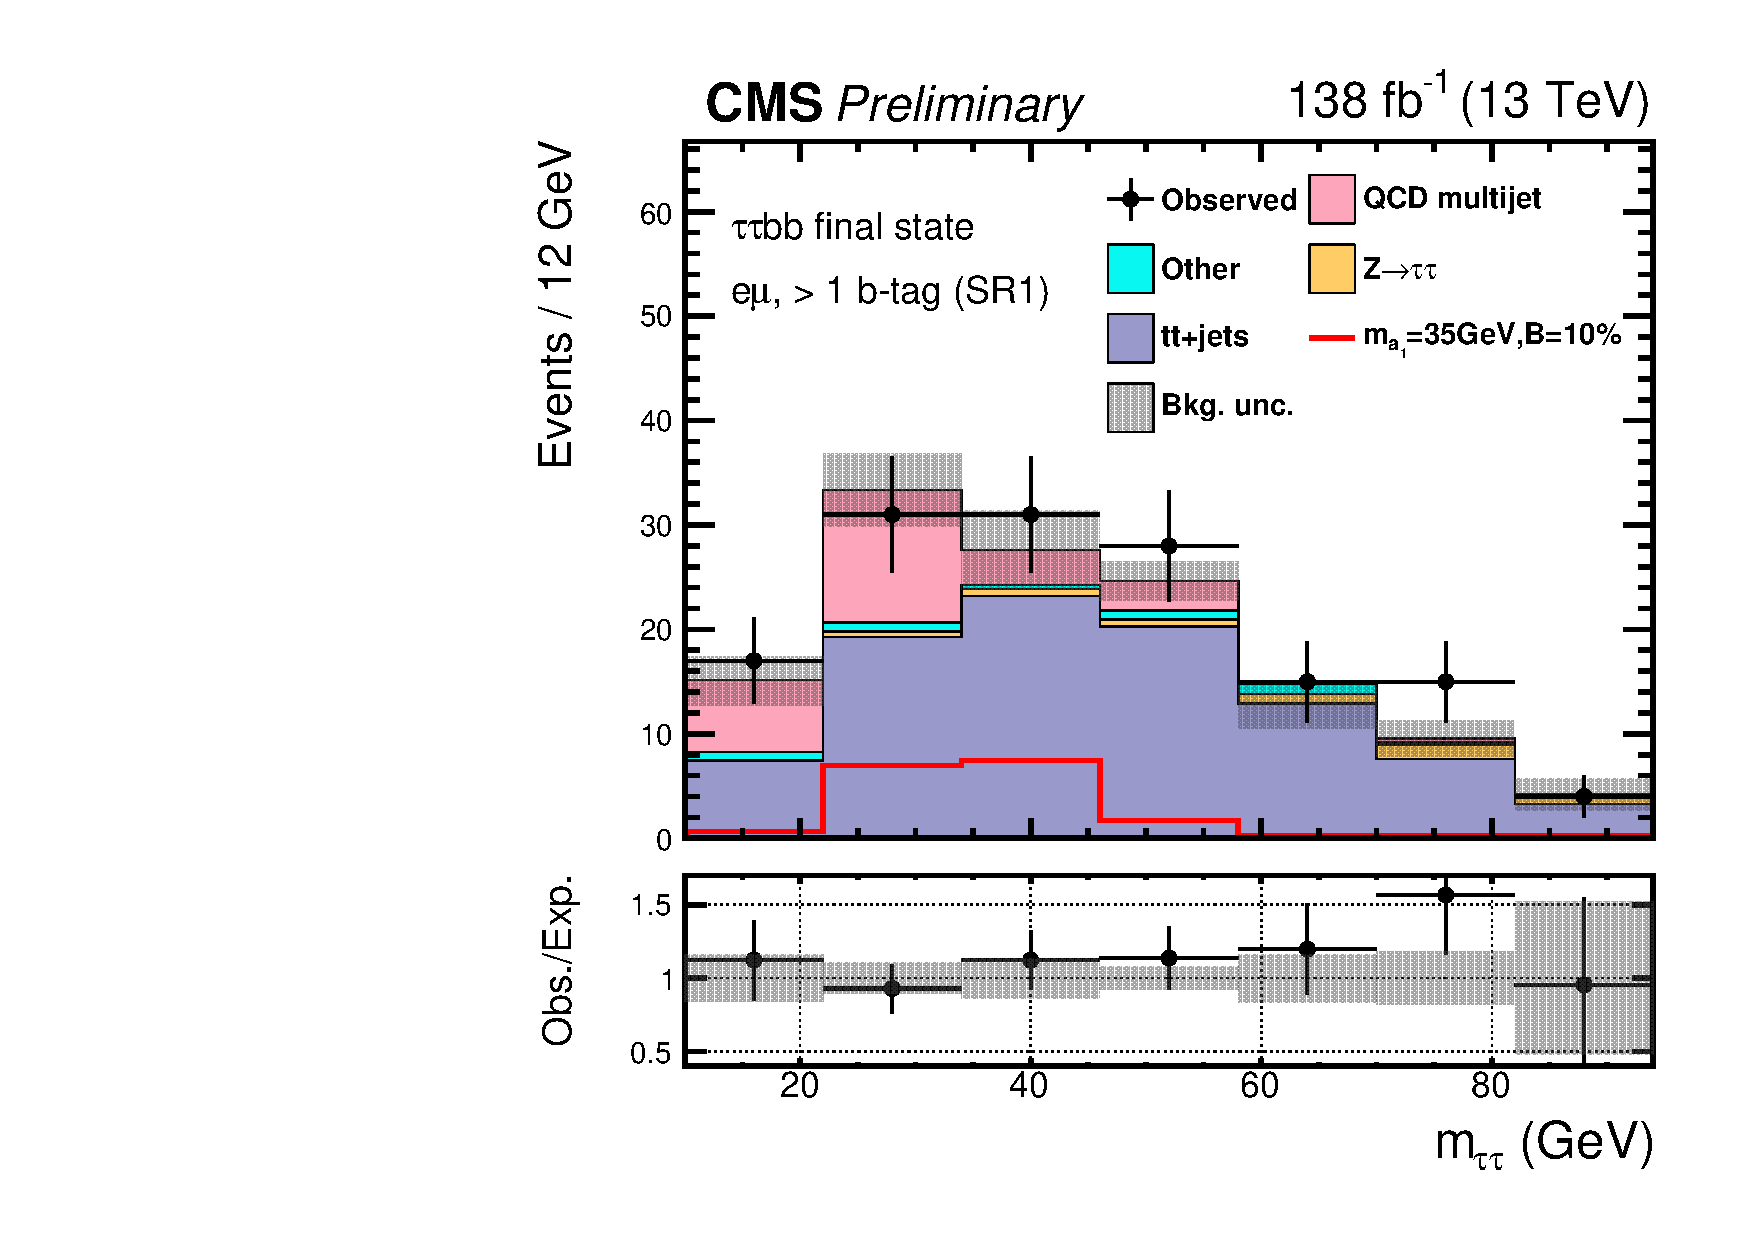
\includegraphics[width=0.32\textwidth]{figures/ch-14-results/em_all_5_post_prelim-yes.pdf}
        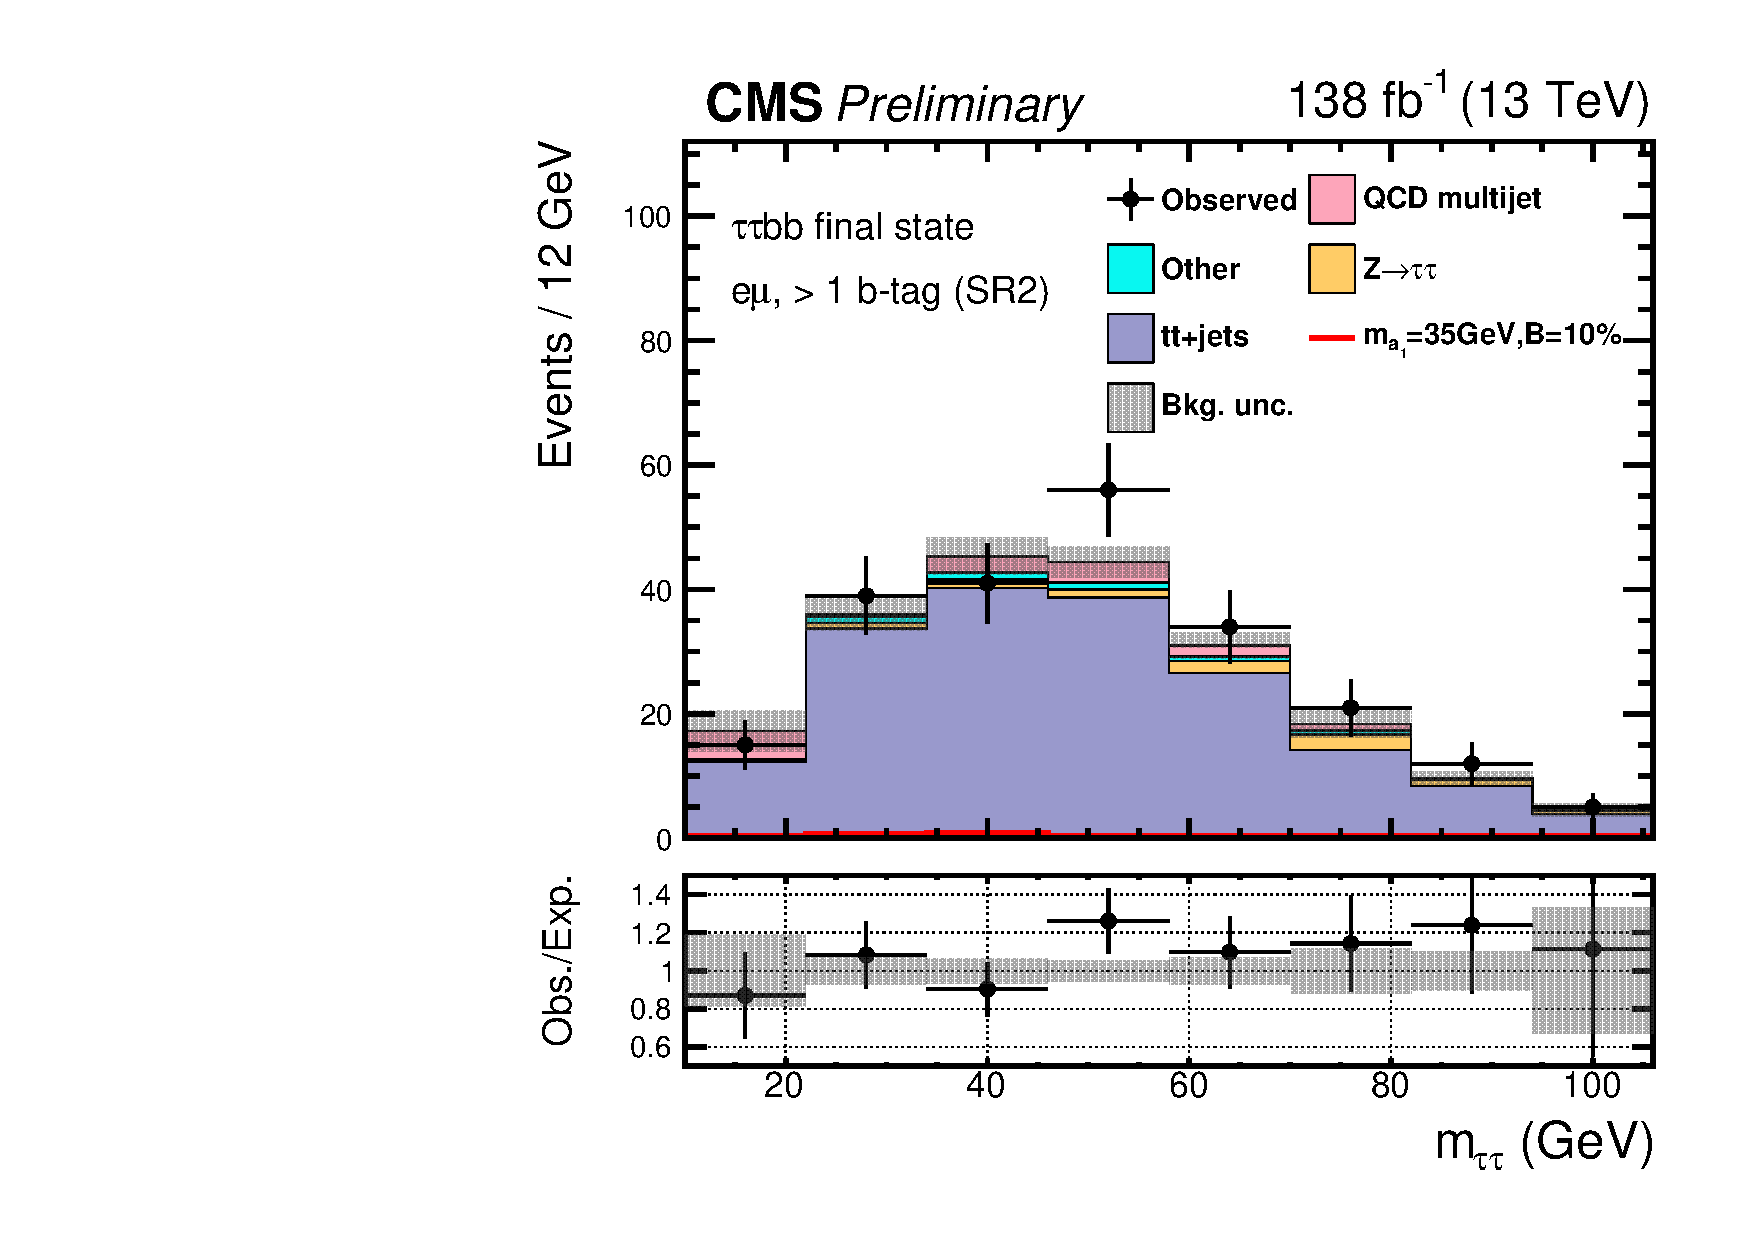
\includegraphics[width=0.32\textwidth]{figures/ch-14-results/em_all_6_post_prelim-yes.pdf}\\
        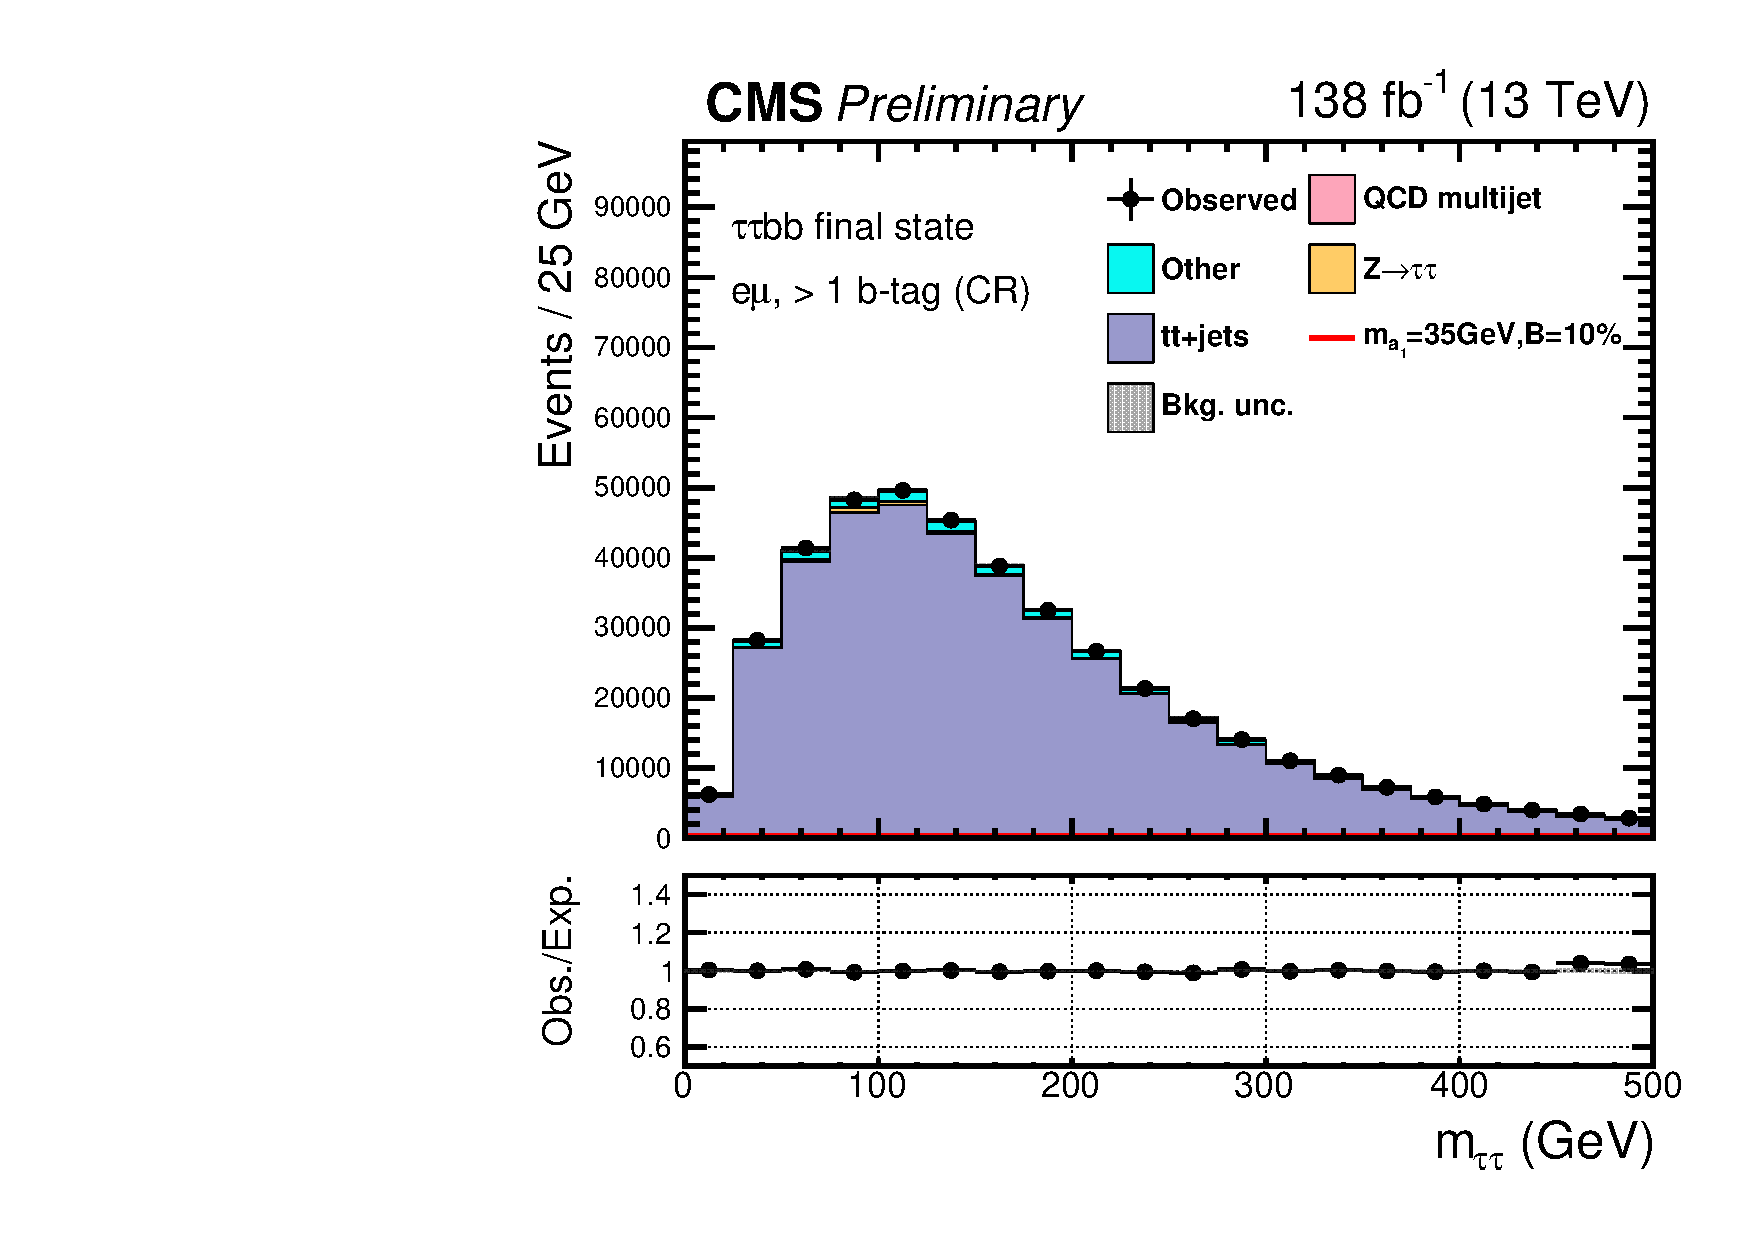
\includegraphics[width=0.32\textwidth]{figures/ch-14-results/em_all_7_post_prelim-yes.pdf}
    \end{center}
    \caption[Postfit final $m_{\tau\tau}$ distributions in the $e\mu$ channel.]{Postfit final $m_{\tau\tau}$ distributions in the $e\mu$ channel \cite{CMS-AN-20-213}. Statistical and systematic uncertainties are included. \textit{Top row:} 1 b-tag jet categories: three signal regions (SR1, SR2, and SR3). \textit{Middle row, left to right:} 1 b-tag jet categories: control region (CR), and 2 b-tag jet categories: signal regions (SR1 and SR2). \textit{Bottom:} 2 b-tag jet categories: control region (CR).}
    \label{fig:results_mtt_postfit_emall}
\end{figure}


The 95\% CL exclusion limits on the signal strength of the branching ratio $\mathcal{B}(h \rightarrow aa \rightarrow bb\tau\tau)$, shown in percentage and normalized to the Standard Model Higgs production cross-section, is shown in Fig. \ref{fig:results_limits}. The pseudoscalar mass hypotheses $m_a$ between 15 GeV and 60 GeV are searched for in all channels. The $e\mu$ channel is the only channel that can provide sensitivity to the $m_a = 12$ GeV mass point, as its cut on the $\Delta R$ between the two $\tau$ legs is the smallest, which increases the signal acceptance for low mass signals.

No excess of events above the Standard Model expectations is observed. Combined expected (observed) limits between 1.4 and 5.6\% (1.7 and 7.6\%) are set for the pseudoscalar mass range between 12 and 60 GeV. The best sensitivity is attained at intermediate mass points, since the analysis targets a resolved signature: at low mass points, objects have a boosted signature, and at high mass points, the $m_{\tau\tau}$ distributions in signal have larger overlap with background distributions.

\begin{figure}[h!]
    \begin{center}
        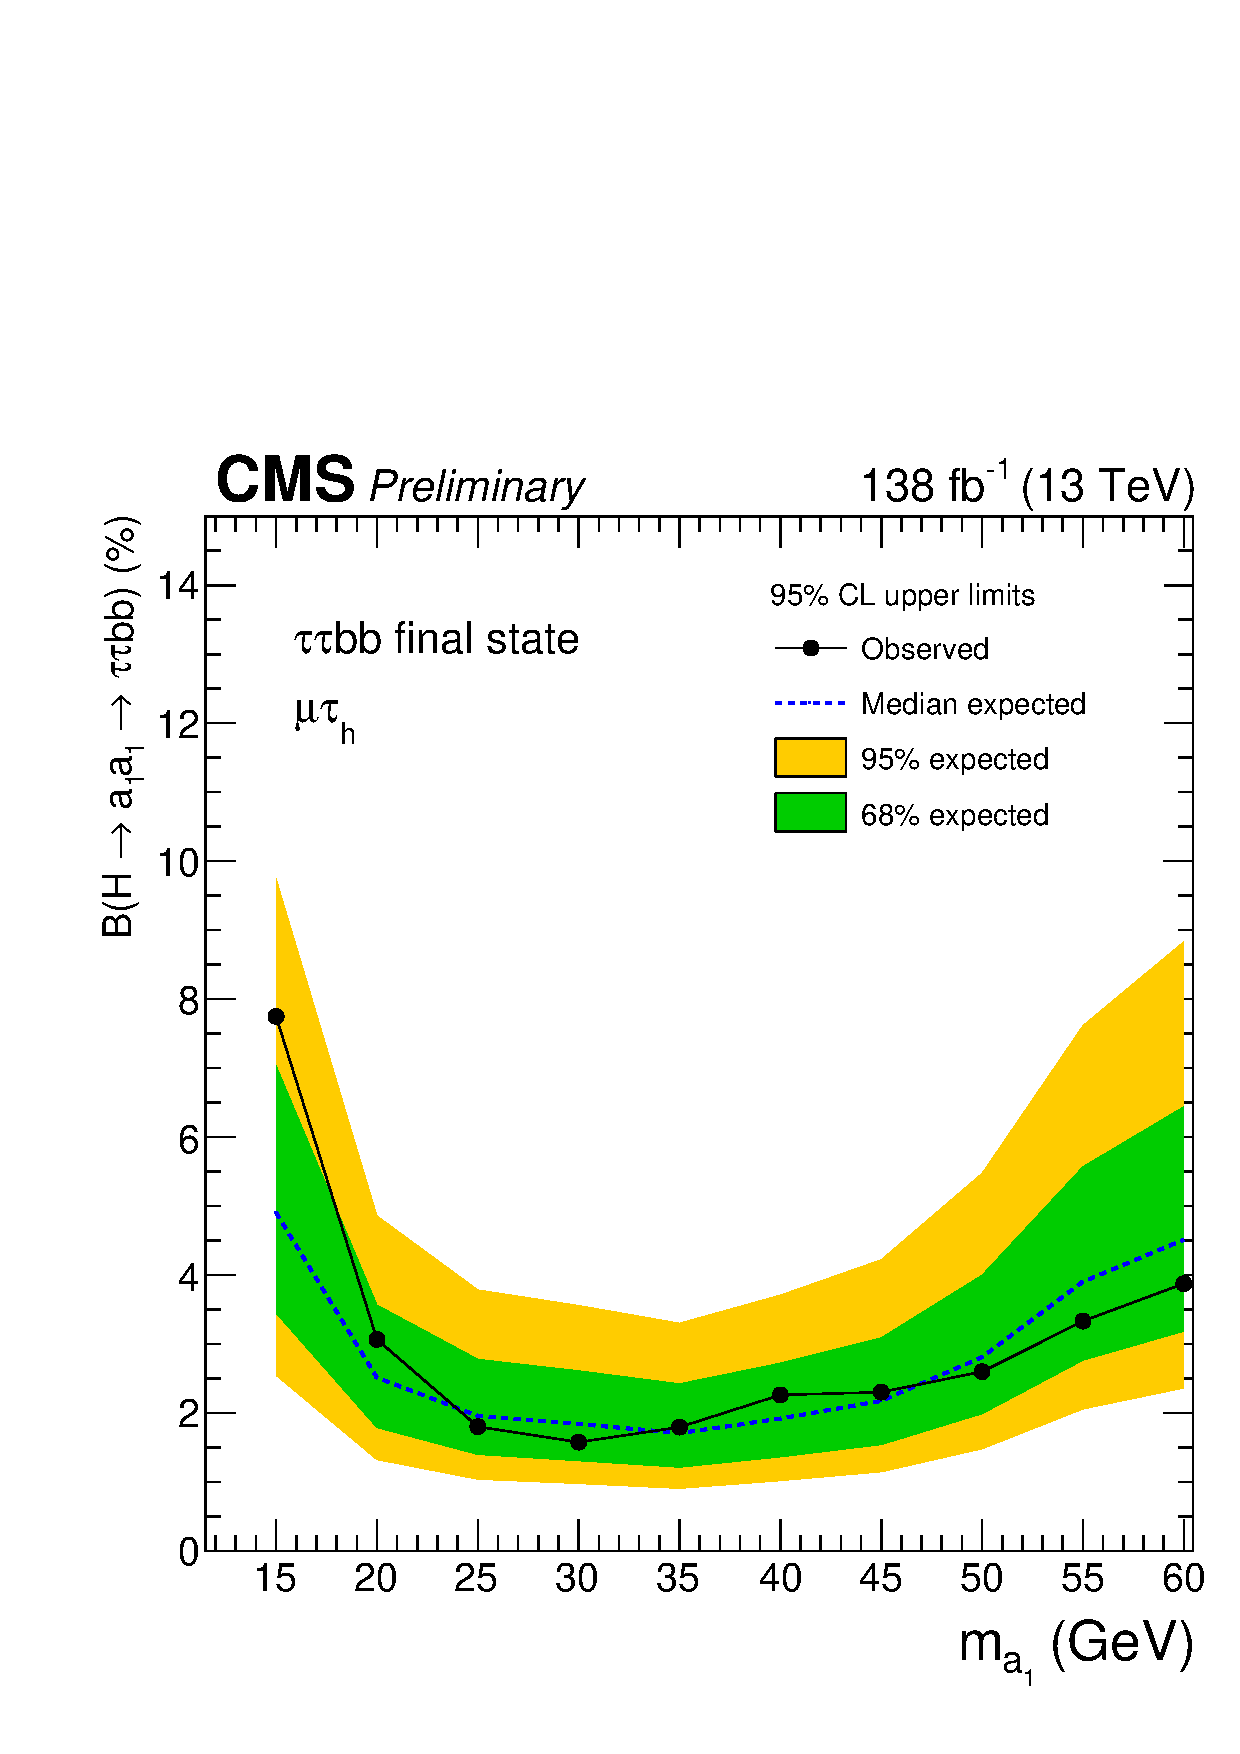
\includegraphics[width=0.45\textwidth]{figures/ch-14-results/Limit_mt_prelim.pdf}
        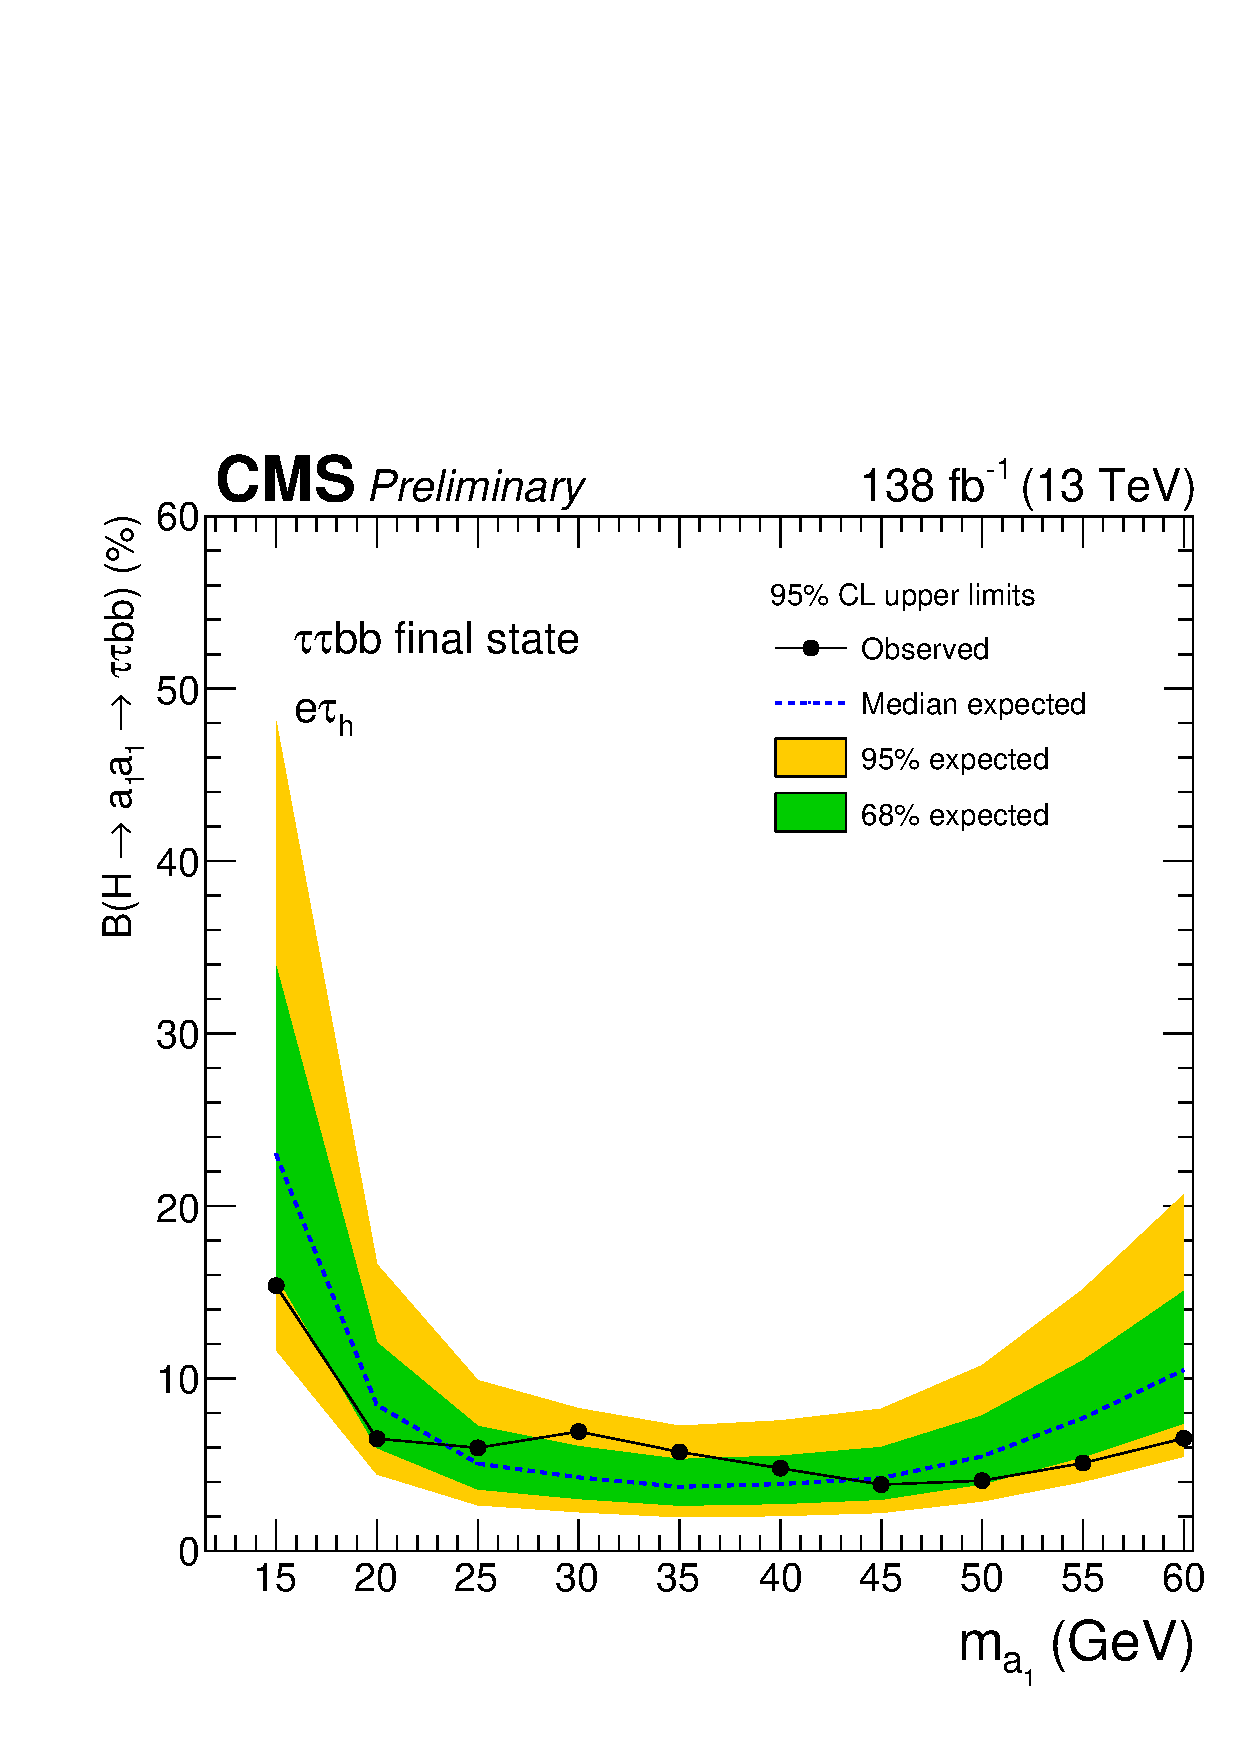
\includegraphics[width=0.45\textwidth]{figures/ch-14-results/Limit_et_prelim.pdf}\\
        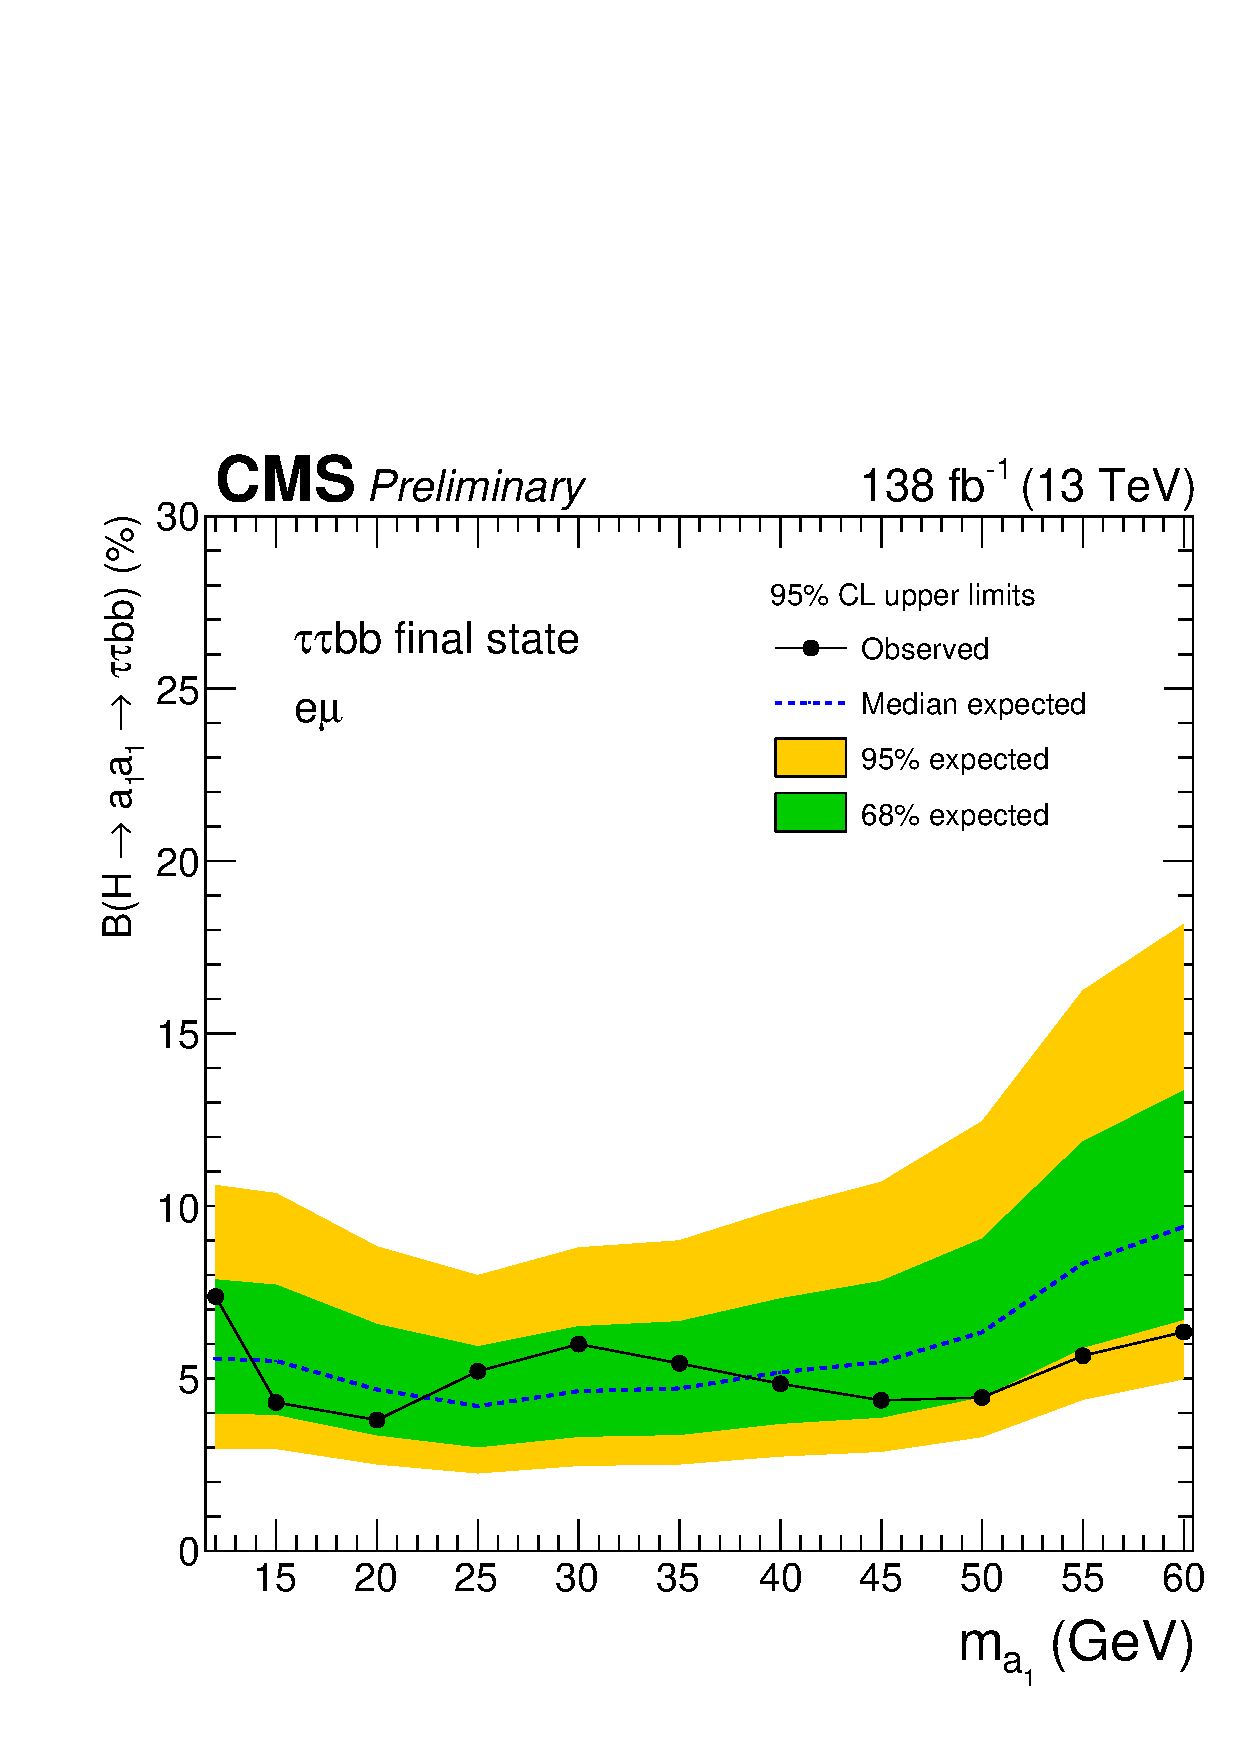
\includegraphics[width=0.45\textwidth]{figures/ch-14-results/Limit_em_prelim.pdf}
        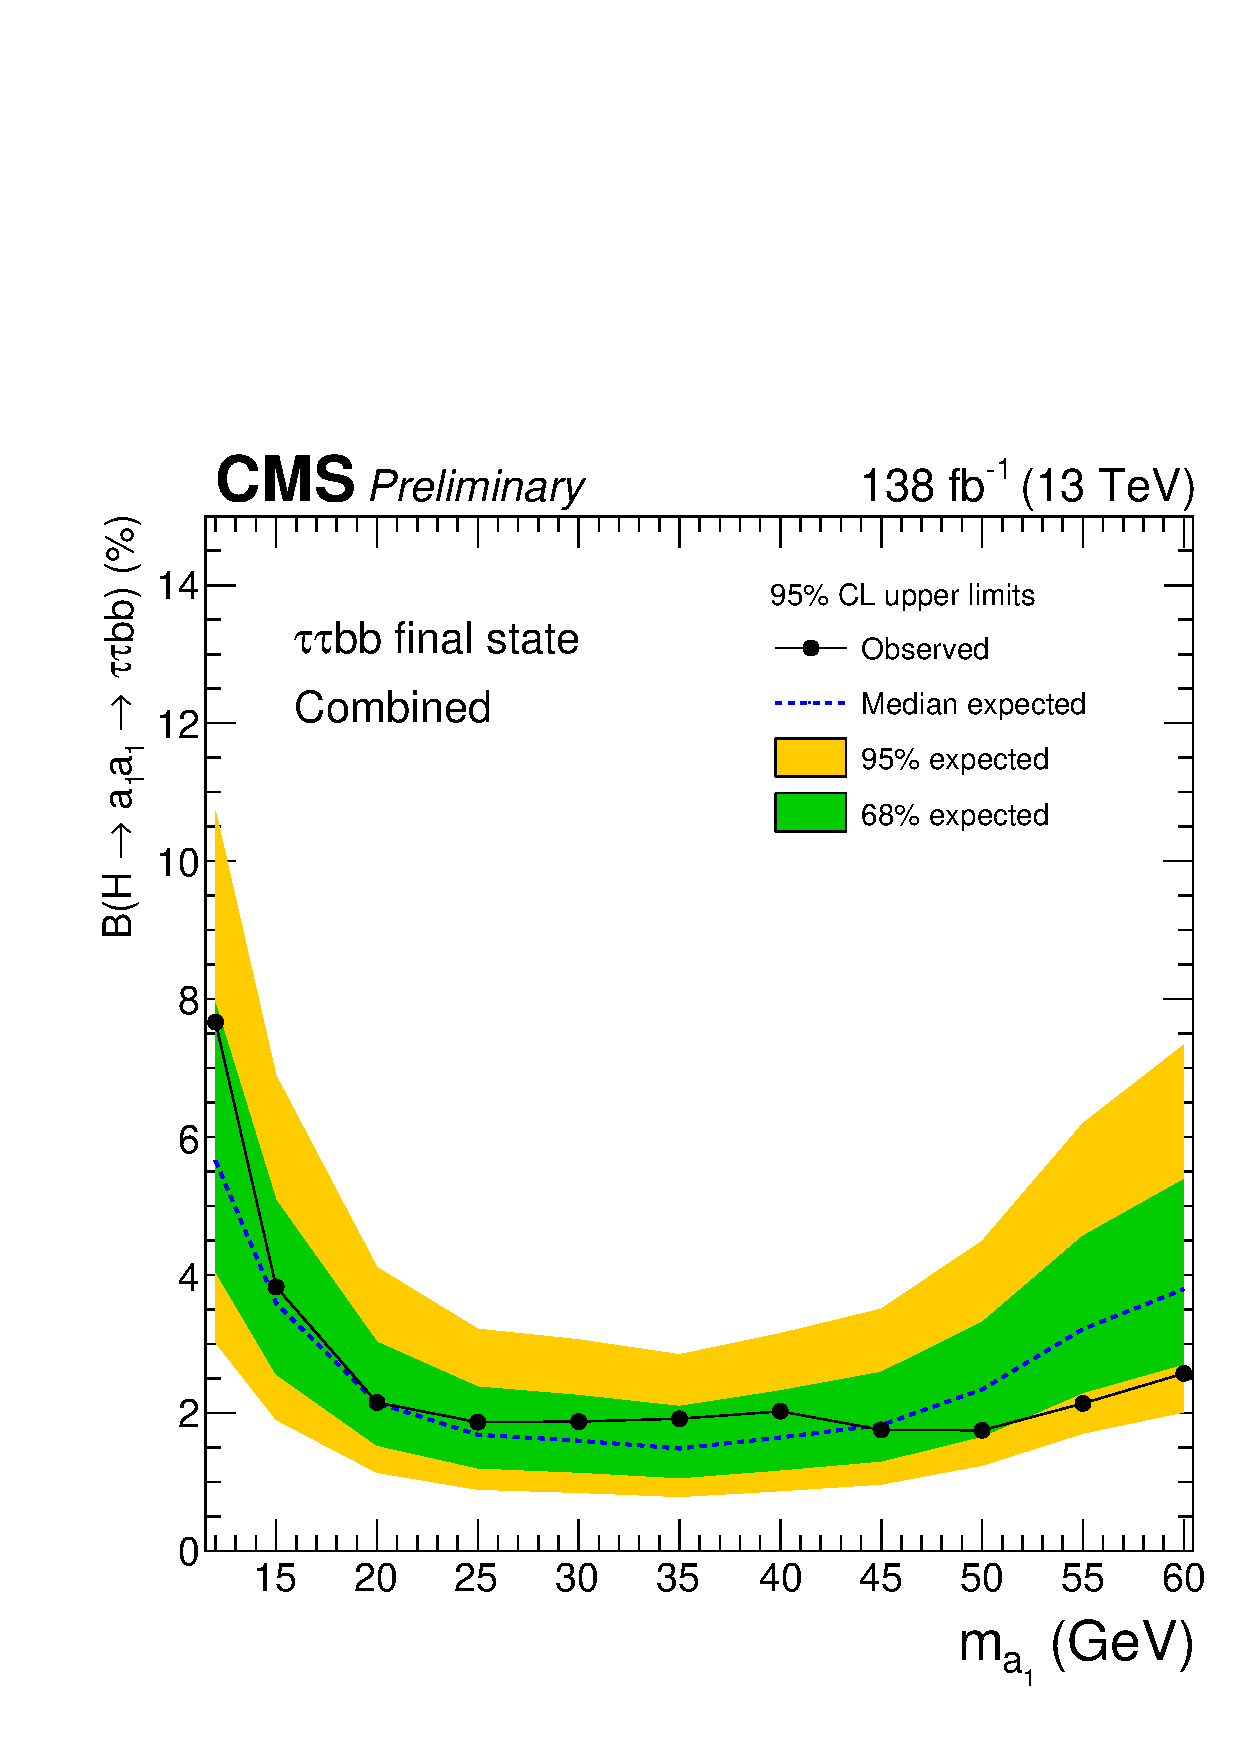
\includegraphics[width=0.45\textwidth]{figures/ch-14-results/Limit_all_prelim.pdf}
    \end{center}
    \caption[95\% CL exclusion limits on B($h\rightarrow aa\rightarrow bb\tau\tau$) in \%.]{95\% CL exclusion limits on B($h\rightarrow aa\rightarrow bb\tau\tau$) in \%, for the combination of all years by channel (\textit{top left}: $\mu\tau_{h}$ channel, \textit{top right:} $e\tau_{h}$ channel, and \textit{Bottom left:} $e\mu$ channel) and the combination of all channels (\textit{bottom right}) \cite{CMS-AN-20-213}.}
    \label{fig:results_limits}
\end{figure}

The branching fraction of the two pseudoscalars depends on the 2HDM+S model type, the pseudoscalar mass $m_a$, and the ratio of the two vacuum expectation values $\tan\beta$. In Type I models, the branching fraction is independent of $\tan\beta$, while in Type III and IV models, it is a function of $m_a$ and $\tan\beta$. Using the predicted values of $B(a \rightarrow ff)$, the observed limits can be used to constrain the $\tan\beta$ vs. $m_a$ phase space. 


\section{Combination procedure with $bb\mu\mu$ final state}
\label{section:ch-13-combination-procedure-with-bbmumu}
A combination of the results from $bb\tau\tau$ is performed with the analysis for the $h \rightarrow aa \rightarrow bb\mu\mu$ final state \cite{CMS-AN-21-058-bbmumu}. While the $bb\mu\mu$ final state has a small branching ratio, it provides competitive results due to the excellent di-muon resolution measured by CMS. The $bb\mu\mu$ analysis uses an unbinned fit to the data using the di-muon mass $m_{\mu\mu}$ distribution.

A combination is possible because the two final states use event selections that are orthogonal to each other, as the $bb\tau\tau$ channels veto events with extra leptons. Several systematic uncertainties are treated as correlated: the integrated luminosity normalization,the b-tagging scale factor, the scale factors related to muon reconstruction, identification, and trigger efficiencies, the inefficiency in the ECAL trigger readout, and the theoretical uncertainties related to signal modeling.

The dimuon and ditau mass distributions ($m_{\mu\mu}$ and $m_{\tau\tau}$) are compared to the data in a combined maximum likelihood fit to derive upper limits on B($h\rightarrow aa$). 

\section{Results from combination}

The observed limits at 95\% CL on B($h \rightarrow aa$) for different 2HDM+S scenarios are shown for the $bb\mu\mu$ analysis in Fig. \ref{fig:results_limits_mmbb}, the $bb\tau\tau$ analysis in Fig. \ref{fig:results_limits_ttbb}, and the combined analyses in Fig. \ref{fig:results_limits_combined}. For 2HDM+S Types II, III, and IV, exclusion limits are set as a function of $\tan\beta$ and $m_{a}$, and are shown in Fig. \ref{fig:results_limits_combined_2D}.

The most stringent constraints are observed for the Type III model, which predicts combined branching fractions between 0.47 and 0.42 for $\tan\beta = 2.0$ and values of $m_{a}$ between 15 and 60 GeV, while the 95\% CL upper limits are between 0.08 and 0.03. For the Type IV model, the predicted branching fractions from theory are between 0.26 and 0.20 for $\tan\beta = 0.6$ for values of $m_{a}$ between 15 and 60 GeV, and the 95\% CL observed upper limits are between 0.12 and 0.05. 

\begin{figure}[ht]
    \begin{center}
      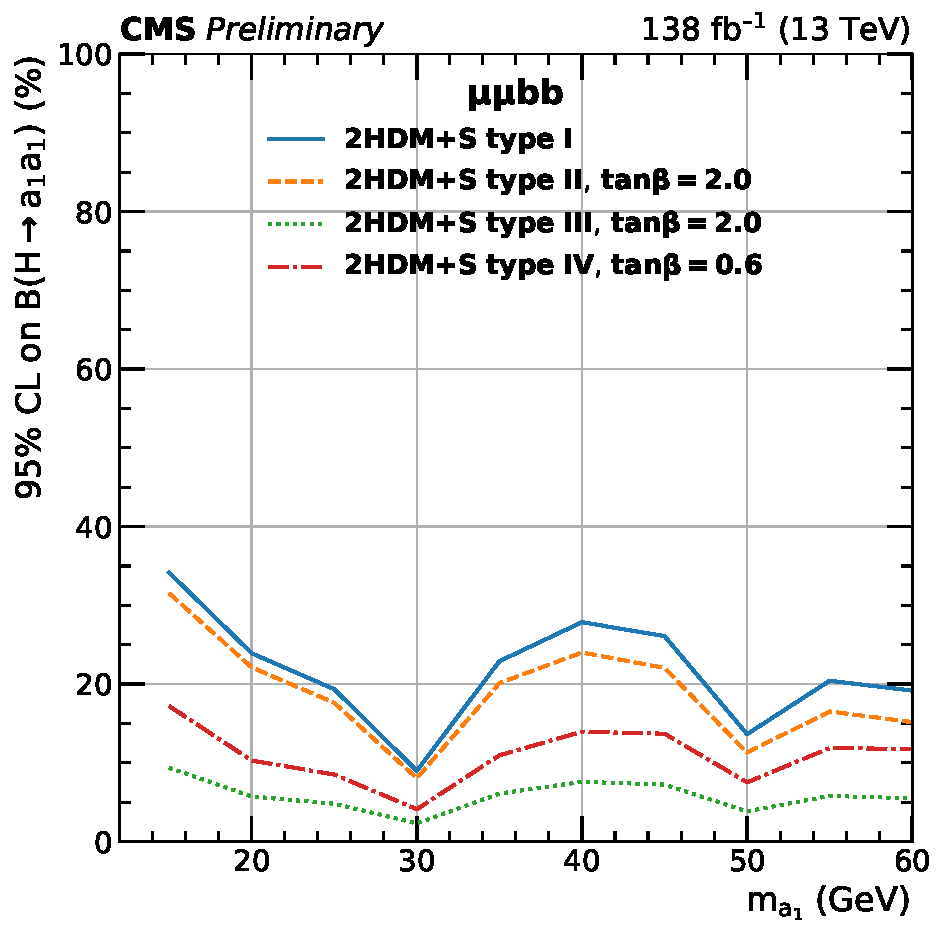
\includegraphics[width=0.5\textwidth]{figures/ch-14-results/HAA_bbmm_all_prelim.pdf}
    \end{center}
    \caption[Observed 95\% CL upper limits on B$(h \rightarrow aa)$ in \%, for the $bb\mu\mu$ channel using the full Run 2 integrated luminosity of 138 $fb^{-1}$ for different 2HDM+S models.]{Observed 95\% CL upper limits on B$(h \rightarrow aa)$ in \%, for the $bb\mu\mu$ channel using the full Run 2 integrated luminosity of 138 $fb^{-1}$ for different 2HDM+S models. Limits on the Type I 2HDM+S model do not depend on $\tan\beta$ \cite{CMS-AN-20-213}.}
      \label{fig:results_limits_mmbb}
  \end{figure}
  \begin{figure}[h!]
    \begin{center}
      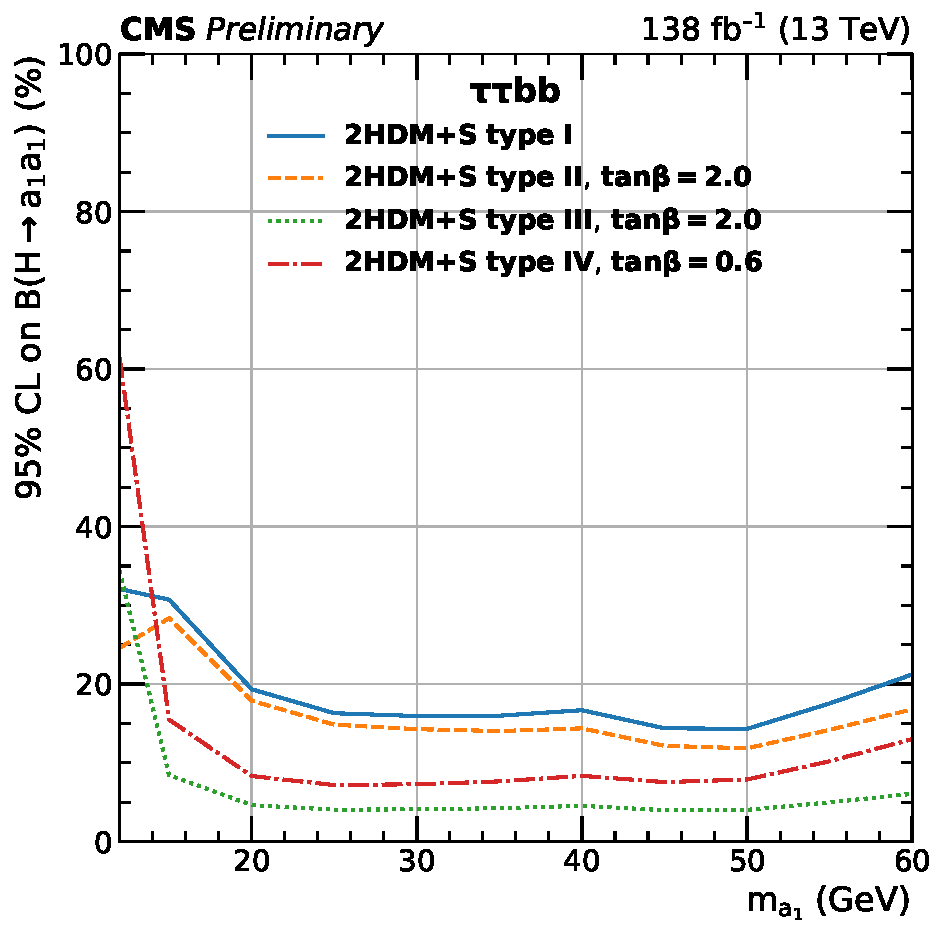
\includegraphics[width=0.5\textwidth]{figures/ch-14-results/HAA_bbtt_all_prelim.pdf}
    \end{center}
    \caption[Observed 95\% CL upper limits on B$(h \rightarrow aa)$ in \%, for the $bb\tau\tau$ channel using the full Run 2 integrated luminosity of 138 $fb^{-1}$ for different 2HDM+S models.]{Observed 95\% CL upper limits on B$(h \rightarrow aa)$ in \%, for the $bb\tau\tau$ channel using the full Run 2 integrated luminosity of 138 $fb^{-1}$ for different 2HDM+S models. Limits on the Type I 2HDM+S model do not depend on $\tan\beta$ \cite{CMS-AN-20-213}.}
      \label{fig:results_limits_ttbb}
  \end{figure}
  \begin{figure}[h!]
    \begin{center}
      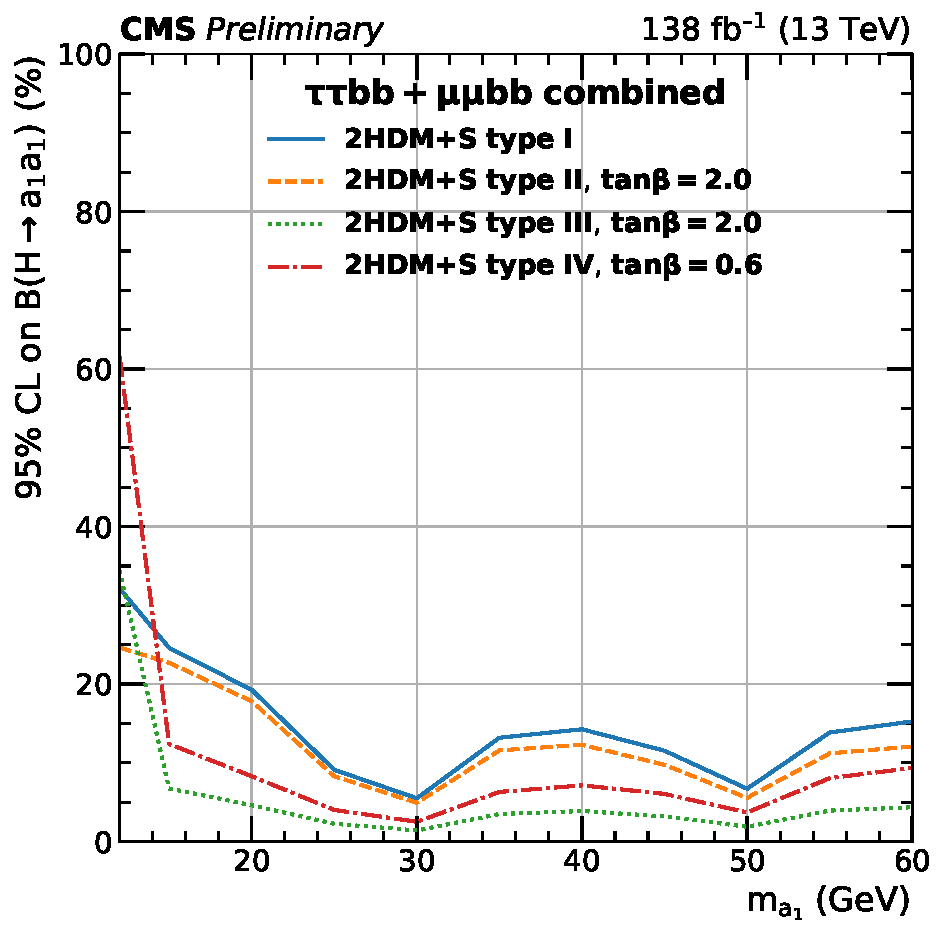
\includegraphics[width=0.5\textwidth]{figures/ch-14-results/HAA_comb_all_prelim.pdf}
    \end{center}
    \caption[Observed 95\% CL upper limits on $\mathcal{B}(h\to aa)$ in \%, for the combination of $bb\mu\mu$ and $bb\tau\tau$ channels using the full Run 2 integrated luminosity of 138 $fb^{-1}$ for different 2HDM+S models.]{Observed 95\% CL upper limits on $\mathcal{B}(h\to aa)$ in \%, for the combination of $bb\mu\mu$ and $bb\tau\tau$ channels using the full Run 2 integrated luminosity of 138 $fb^{-1}$ for different 2HDM+S models. Limits on the Type I 2HDM+S model do not depend on $\tan\beta$ \cite{CMS-AN-20-213}.}
      \label{fig:results_limits_combined}
  \end{figure}
  


\begin{figure}[h]
    \begin{center}
      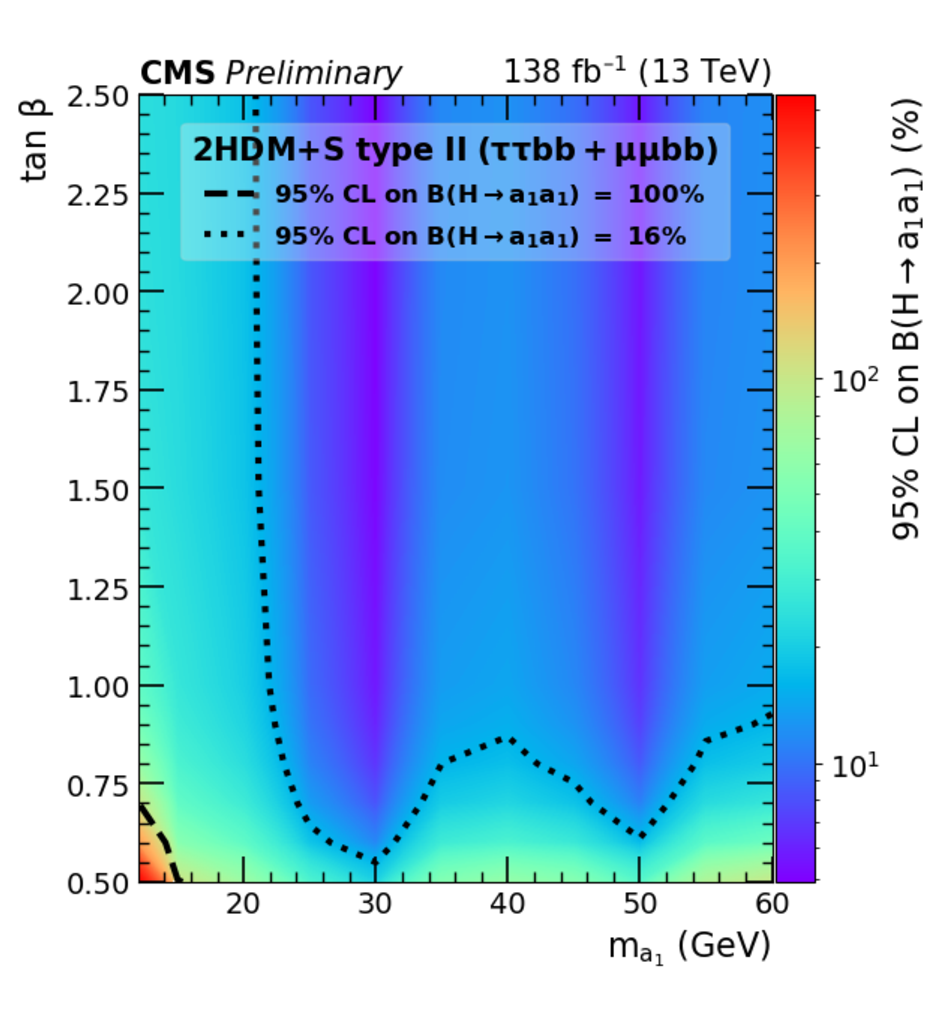
\includegraphics[width=0.32\textwidth]{figures/ch-14-results/HAA_comb_II_prelim.pdf}
      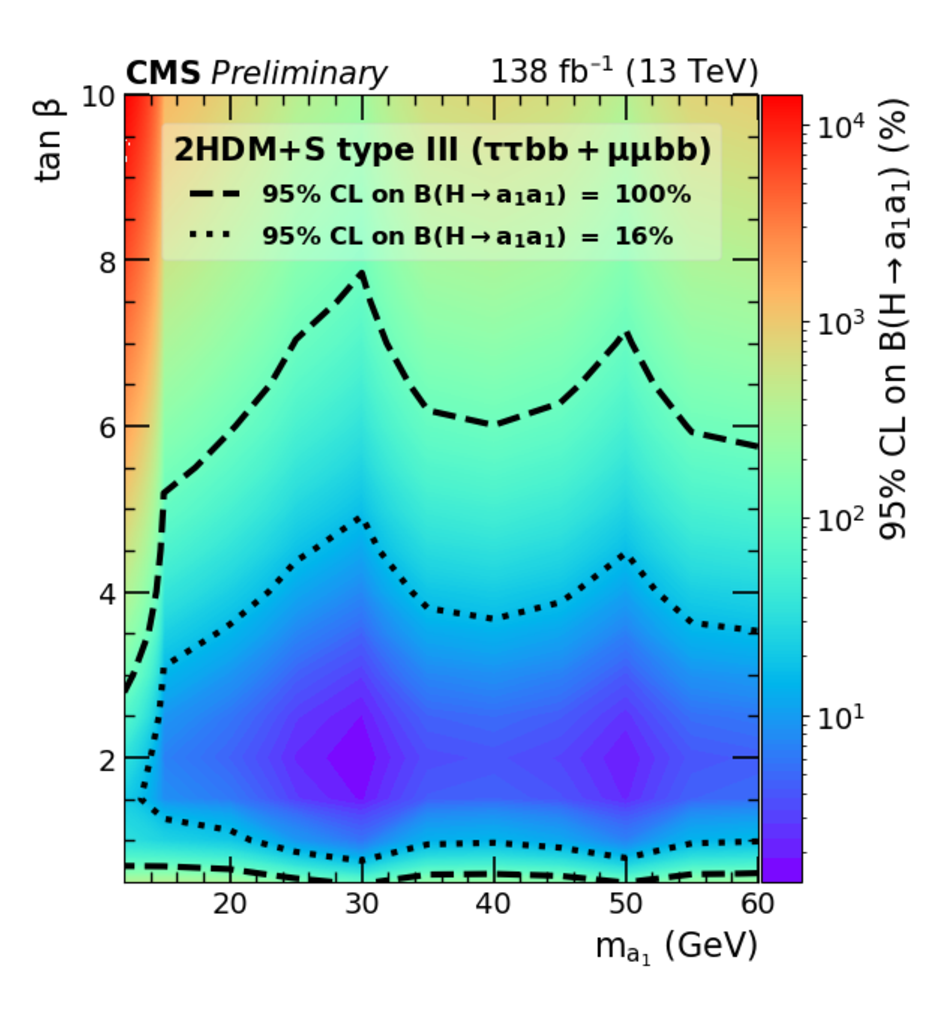
\includegraphics[width=0.32\textwidth]{figures/ch-14-results/HAA_comb_III_prelim.pdf}
      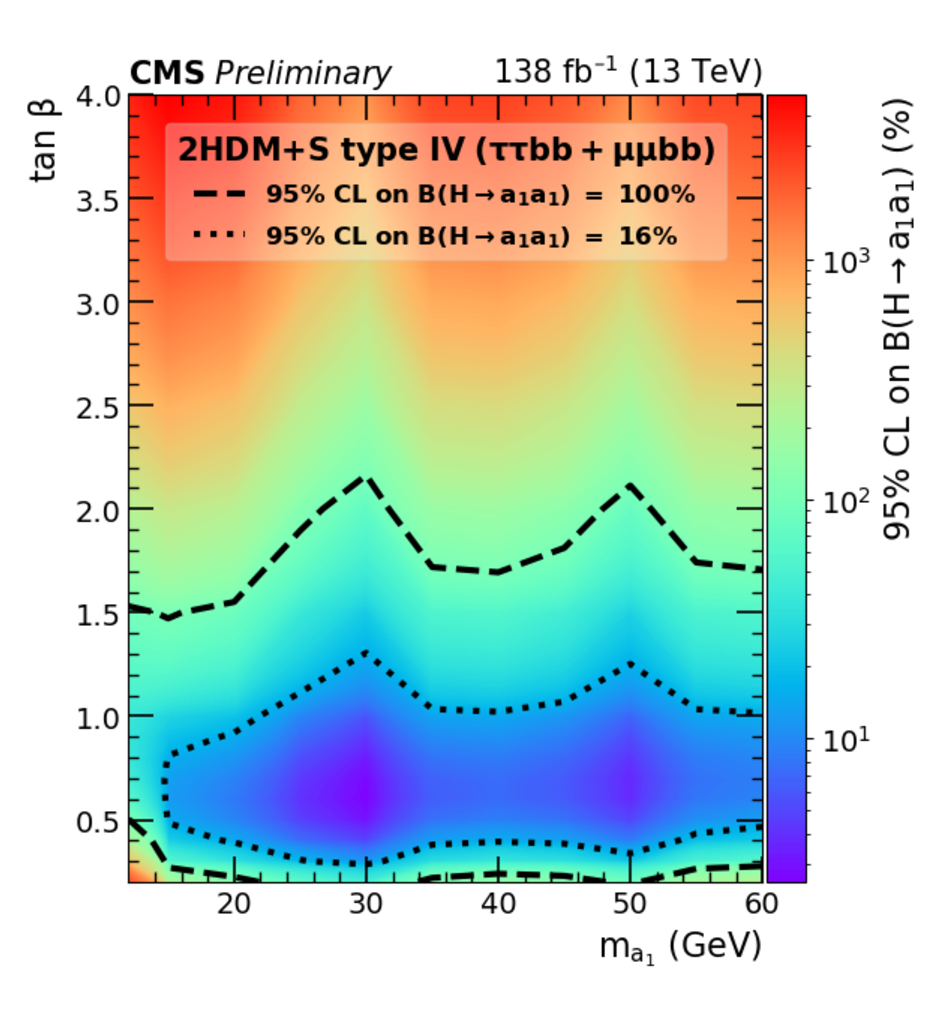
\includegraphics[width=0.32\textwidth]{figures/ch-14-results/HAA_comb_IV_prelim.pdf}
    \end{center}
    \caption[Observed 95\% CL upper limits on $\mathcal{B}(h\to aa)$ in \%, for the combination of $bb\mu\mu$ and $bb\tau\tau$ channels using the full Run 2 integrated luminosity of 138 $fb^{-1}$ for Type II (\textit{left}), Type III (\textit{middle}), and Type IV (\textit{right}) 2HDM+S in the $\tan\beta$ vs. $m_a$ phase space.]{Observed 95\% CL upper limits on $\mathcal{B}(h\to aa)$ in \%, for the combination of $bb\mu\mu$ and $bb\tau\tau$ channels using the full Run 2 integrated luminosity of 138 $fb^{-1}$ for Type II (\textit{left}), Type III (\textit{middle}), and Type IV (\textit{right}) 2HDM+S in the $\tan\beta$ vs. $m_a$ phase space. The contours corresponding to branching ratios of 100\% and 34\% are drawn using dashed lines, 34\% corresponding to the previous upper limit on Higgs to BSM particle decays during Run 1. Linear extrapolation has been used between different points on the figures \cite{CMS-AN-20-213}.}
      \label{fig:results_limits_combined_2D}
  \end{figure}
  
The combined analyses' results are also shown in summary plots alongside the other current CMS results for 2HDM+S limits: for type I in Fig. \ref{fig:summary_plot_type_I}, for type II with $\tan\beta = 2.0$ in Fig. \ref{fig:summary_plot_typeII_tan_beta_2p0}, and for type III with $\tan\beta = 2.0$ in Fig. \ref{fig:summary_plot_typeIII_tan_beta_2p0}. In other scenarios, e.g. type III with $\tan\beta = 5.0$, more stringent limits are set by analyses in other final states, $\mu\mu\tau\tau$ in this case. Other summary plots can be found at \cite{twiki_2HDM+S_summary-plots}.

\begin{figure}[h]
    \begin{center}
      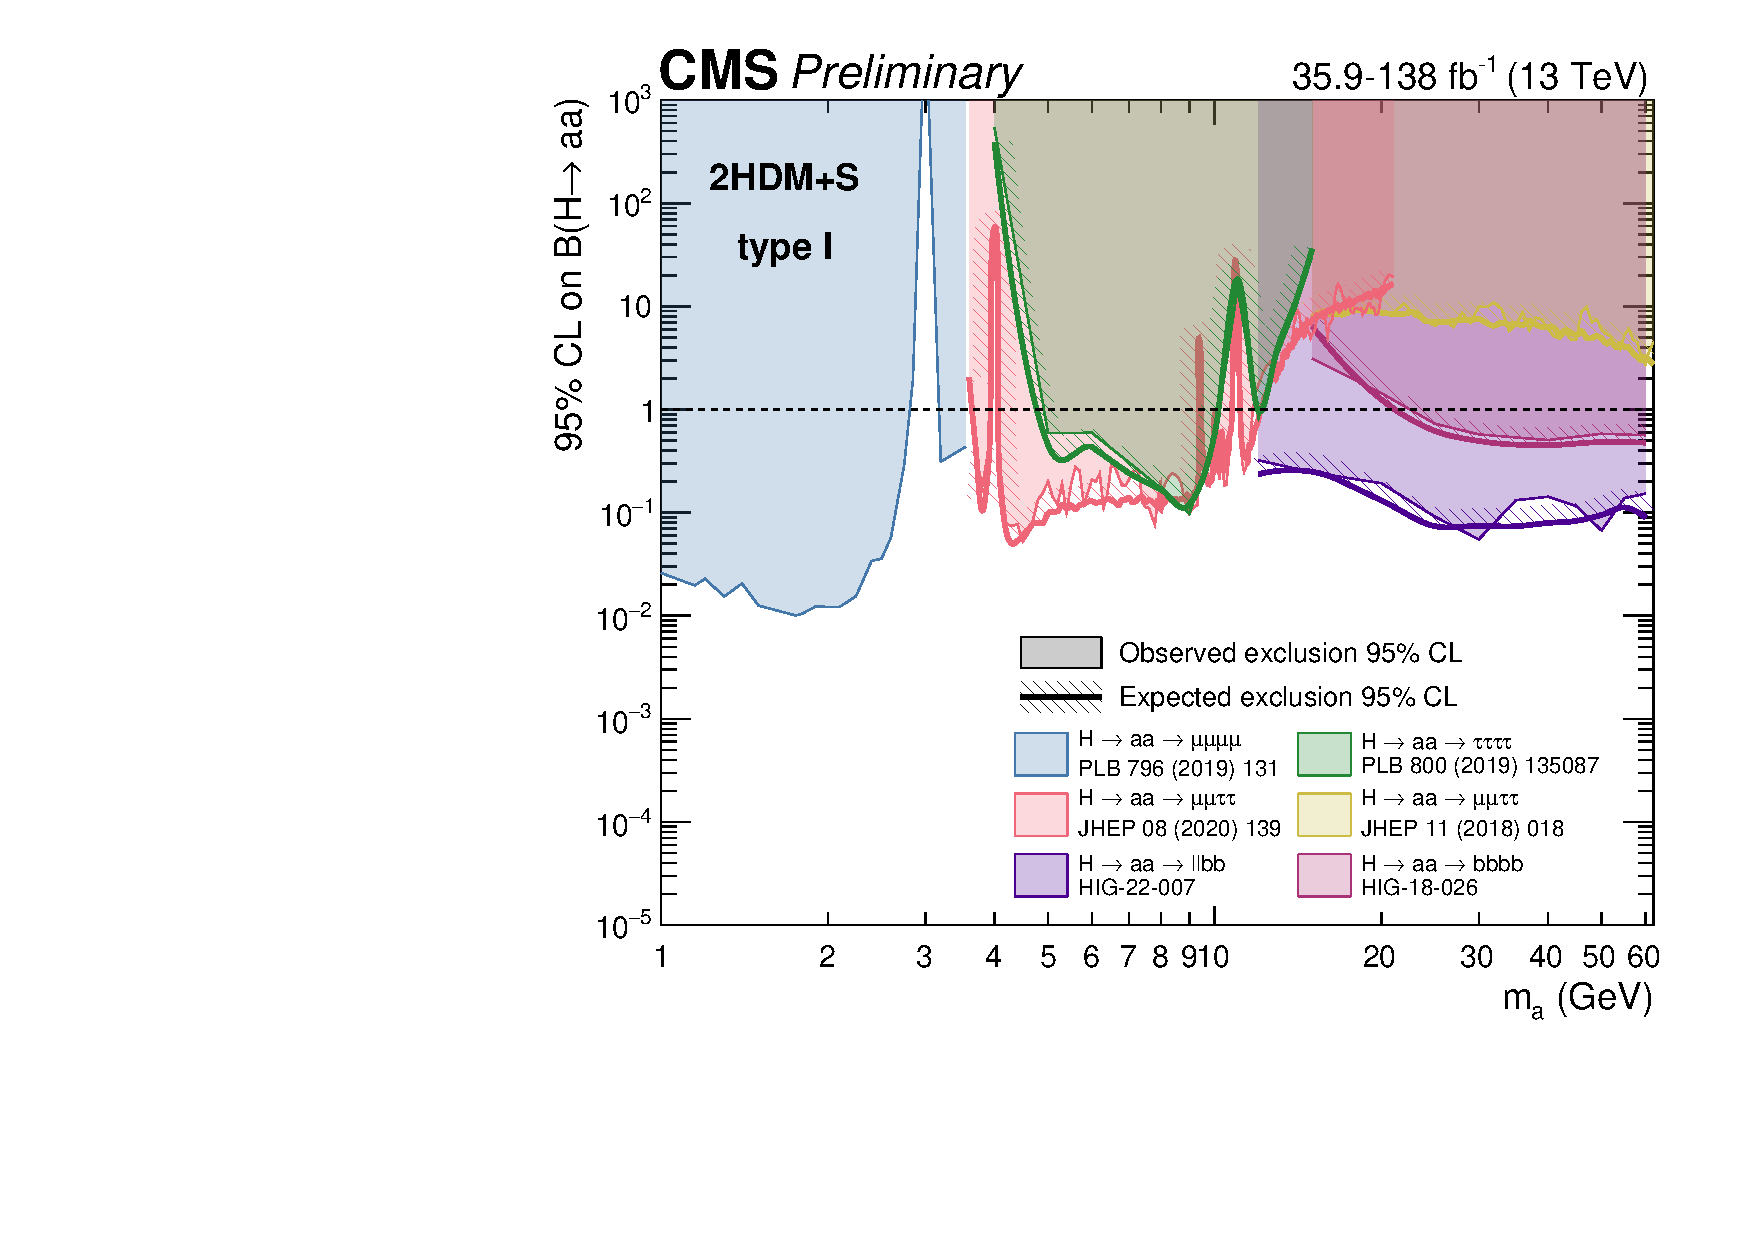
\includegraphics[width=0.6\textwidth]{figures/ch-14-results/summary_plot_full_run2_plot_BRaa_Type1.pdf}
    \end{center}
    \caption[95\% limits on $\frac{\sigma(h)}{\sigma_{\text{SM}}} \times \mathcal{B}(h \rightarrow aa)$ in the 2HDM+S type-I scenario for exotic Higgs decay searches, performed with data collected at 13 TeV.]{95\% limits on $\frac{\sigma(h)}{\sigma_{\text{SM}}} \times \mathcal{B}(h \rightarrow aa)$ in the 2HDM+S type-I scenario for exotic Higgs decay searches, performed with data collected at 13 TeV. The combined result for $h\rightarrow aa \rightarrow \ell\ell bb$ \cite{CMS-HIG-22-007} is shown in purple.}
      \label{fig:summary_plot_type_I}
  \end{figure}
  \begin{figure}[h]
    \begin{center}
      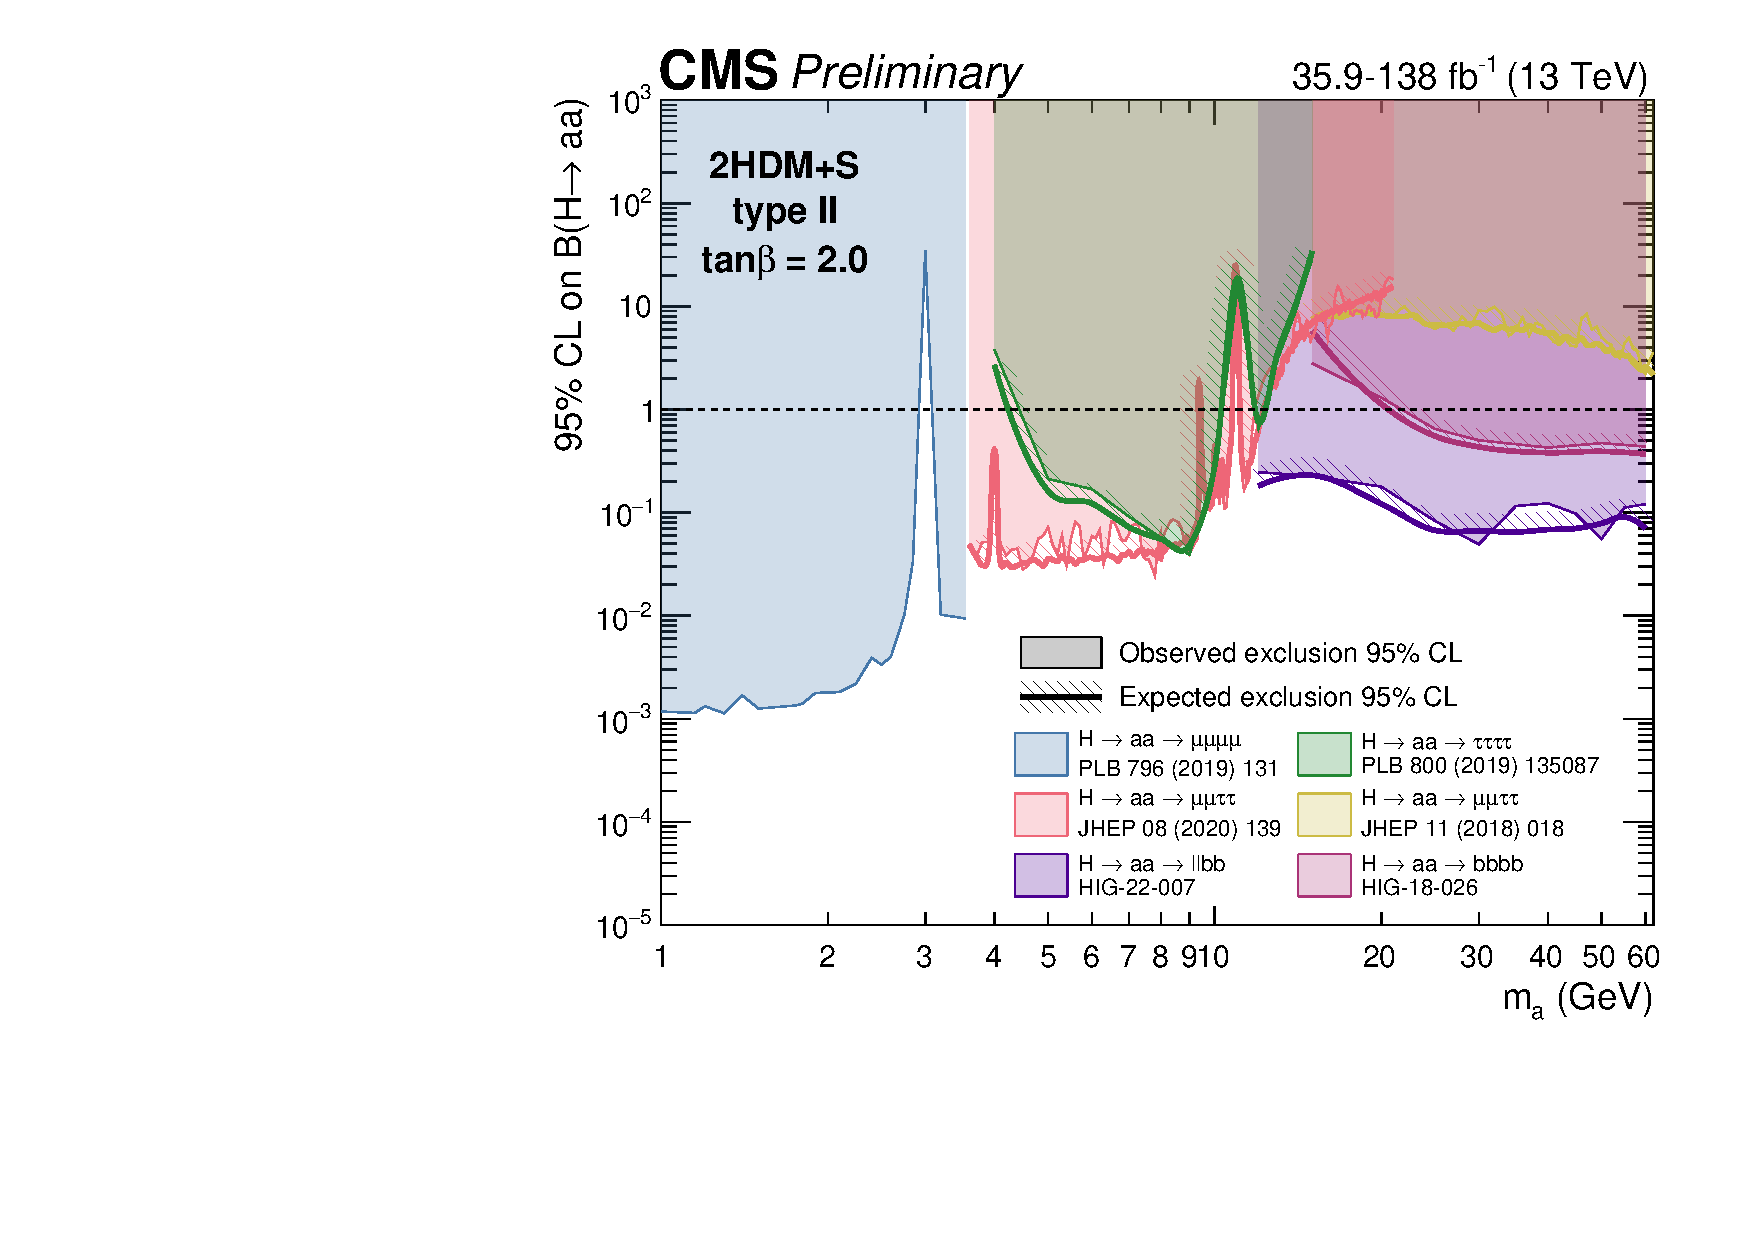
\includegraphics[width=0.6\textwidth]{figures/ch-14-results/summary_plot_full_run2_plot_BRaa_Type2_tanbeta2.pdf}
    \end{center}
    \caption[95\% limits on $\frac{\sigma(h)}{\sigma_{\text{SM}}} \times \mathcal{B}(h \rightarrow aa)$ in the 2HDM+S type-II scenario with $\tan\beta = 2.0$ for exotic Higgs decay searches, performed with data collected at 13 TeV.]{95\% limits on $\frac{\sigma(h)}{\sigma_{\text{SM}}} \times \mathcal{B}(h \rightarrow aa)$ in the 2HDM+S type-II scenario with $\tan\beta = 0.0$ for exotic Higgs decay searches, performed with data collected at 13 TeV. The combined result for $h\rightarrow aa \rightarrow \ell\ell bb$ \cite{CMS-HIG-22-007} is shown in purple, representing the most stringent limits in the probed mass ranges in this scenario.}
      \label{fig:summary_plot_typeII_tan_beta_2p0}
  \end{figure}
  \begin{figure}[h]
    \begin{center}
      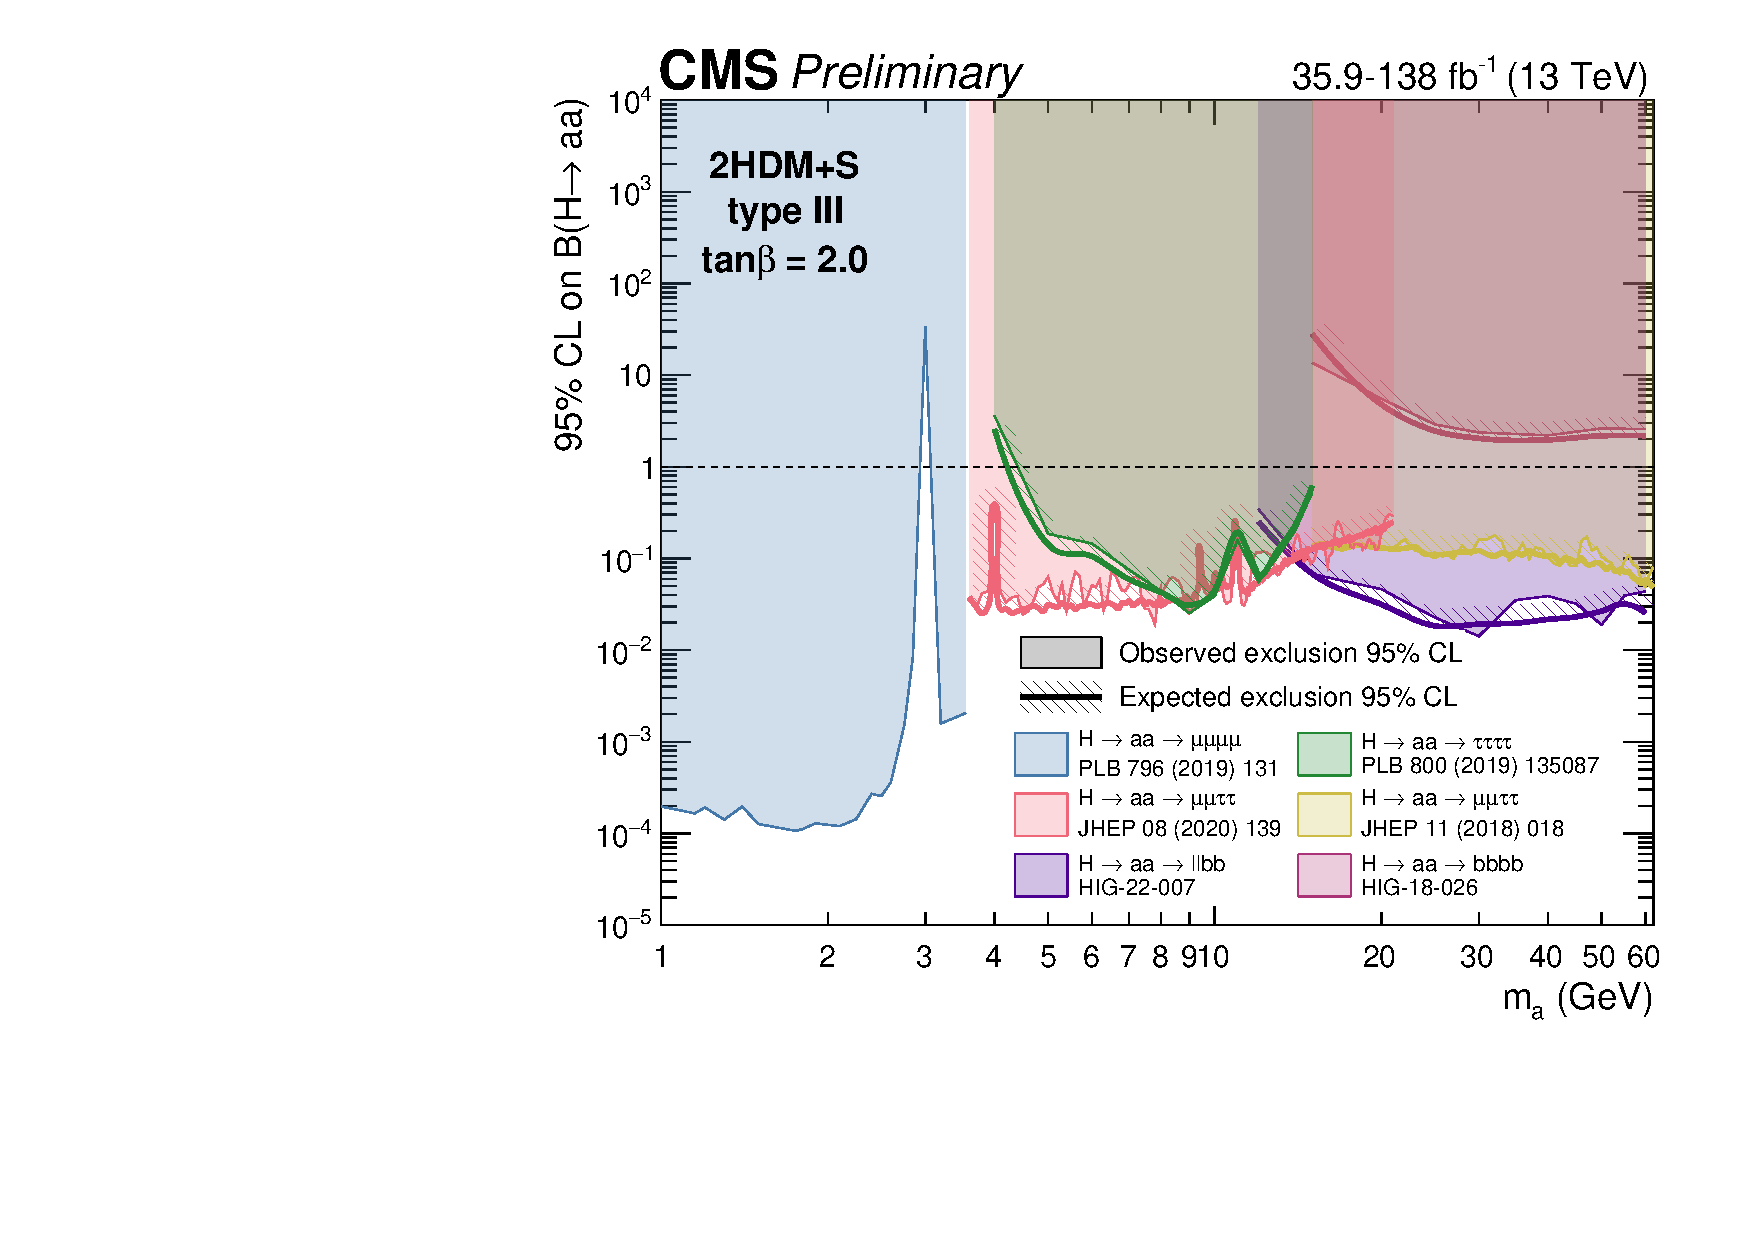
\includegraphics[width=0.6\textwidth]{figures/ch-14-results/summary_plot_full_run2_plot_BRaa_Type3_tanbeta2.pdf}
    \end{center}
    \caption[95\% limits on $\frac{\sigma(h)}{\sigma_{\text{SM}}} \times \mathcal{B}(h \rightarrow aa)$ in the 2HDM+S type-III scenario with $\tan\beta = 2.0$ for exotic Higgs decay searches, performed with data collected at 13 TeV.]{95\% limits on $\frac{\sigma(h)}{\sigma_{\text{SM}}} \times \mathcal{B}(h \rightarrow aa)$ in the 2HDM+S type-III scenario with $\tan\beta = 2.0$ for exotic Higgs decay searches, performed with data collected at 13 TeV. The combined result for $h\rightarrow aa \rightarrow \ell\ell bb$ \cite{CMS-HIG-22-007} is shown in purple.}
      \label{fig:summary_plot_typeIII_tan_beta_2p0}
  \end{figure}
  
